\documentclass[%
%draft,
11pt,%
twoside,%
titlepage,%
swissgerman,%
headsepline%
]{scrartcl}

\usepackage{lastpage}
\usepackage{amsthm}
\usepackage{amssymb}
\usepackage{geometry}
\usepackage{graphicx}
\usepackage[dvipsnames]{xcolor}
\usepackage[utf8]{inputenc}
\usepackage[swissgerman]{babel}
\usepackage{lscape}
\usepackage[framemethod=TikZ]{mdframed}
\usepackage[most]{tcolorbox}
\usepackage{enumerate}
\usepackage{units}
\usepackage{nicefrac}
\usepackage{pgf,tikz}
\usepackage{tikz-3dplot}
\usepackage{tkz-euclide}
\usetikzlibrary{shapes.multipart}
\usetikzlibrary{arrows}
\usetikzlibrary{arrows.meta}
\usetikzlibrary{patterns}
\usetikzlibrary{positioning}
\usetikzlibrary{shadows}
\usetikzlibrary{quotes, angles}
\usepackage{colortbl}
\usepackage{hhline}
\usepackage{multirow}
\usepackage[extendedchars]{grffile}
\usepackage{caption}
\usepackage{multicol,calc}
\usepackage{blindtext}
\usepackage{pdfpages}
\usepackage{hyperref}
\usepackage{framed}
\usepackage{yfonts}
\usepackage{csquotes}

\usepackage{marginnote}
\usepackage{qrcode}
\qrset{height=7ex}

\usepackage{longtable}
\usepackage{listings}
\usepackage{wrapfig}

\usepackage{fontawesome} % Oder FontAwesome, falls du ein Augensymbol aus einer
\newcommand{\faEyeLightGray}{\textcolor{lightgray}{\faEye}} % Custom command for the gray eye icon
\newcommand{\faReturnGray}{\textcolor{gray}{\faMailReply}} % Custom command for the gray eye icon
\usepackage{pifont} % weitere Zeichen

% package für plots mit dem Befehl axes
\usepackage{pgfplots}
\pgfplotsset{compat=1.18}

\usepackage[europeanresistors]{circuitikz}

\usepackage{ifthen}

% Command, um Tabellen-Spalten anzupassen
\newcommand{\spaltenheight}{\rule{0mm}{3ex}}
\newcommand{\spaltenwidth}{\rule{3cm}{0mm}}
\newcommand{\spaltensep}{\\[1ex]}
%\arrayrulecolor{darkgreen}
\doublerulesepcolor{white}

% colors
\definecolor{lightyellow}{rgb}{1,1,0.8}
\definecolor{Gray}{gray}{0.9}
\definecolor{lightgray}{rgb}{0.7, 0.7, 0.7}
\definecolor{darkblue}{rgb}{0,0,0.55}
\definecolor{firebrick}{rgb}{0.7,0.13,0.13}
\definecolor{seagreen}{rgb}{0.18,0.55,0.34}
\definecolor{emerald}{HTML}{50C878} % color of Definition
\definecolor{whitesmoke}{HTML}{F5F5F5} % background for environments
\definecolor{myblizzardblue}{HTML}{87CEEB} % color of Satz

% Für Definitionen im Fliesstext
\newcommand{\definition}[1]{\colorbox{emerald}{#1}}
% Für Regeln im Fliesstext
\newcommand{\regel}[1]{\colorbox{myblizzardblue}{#1}}
% Für Merke/Achtungs im Fliesstext
\newcommand{\merke}[1]{\colorbox{firebrick}{#1}}
% Geogebra-Link
\newcommand{\geogebralink}{\href{https://www.geogebra.org/calculator}{\texttt{geogebra.org}}}

% Umgebungen
\theoremstyle{definition}
    \newtheorem{bsp}{Beispiel}[section] % Beispiele
    \newtheorem{bem}{Bemerkung}[section] % Bemerkungen
\theoremstyle{plain}
    \newtheorem{thm}{Theorem} % Theorem [subsection]
    \newtheorem{satz}{Satz} % Satz [subsection]

% Umgebung lsg mit dynamischer Referenzierung und Label
\newcommand{\concatueb}[1]{ueb:#1}% Definition für concatueb
\newcommand{\concatlsg}[1]{lsg:#1}% Definition für concatlsg

\newcounter{uebcounter}[section]
\renewcommand{\theuebcounter}{\thesection.\arabic{uebcounter}}  % Zählerformat: Abschnitt.Übung

\newenvironment{lsg}[1]{%
    \par\noindent\textbf{Notizen zu Übung \ref{\concatueb{#1}}}\label{\concatlsg{#1}}
    \hfill\hyperref[\concatueb{#1}]{\faReturnGray}\par % Hyperref-Button zurück zur Übung
}{%
    \par%
}

\newenvironment{uebenv}[1]{%
    \refstepcounter{uebcounter}
    \par\noindent\textbf{Übung \theuebcounter.}%
    \label{\concatueb{#1}}\hfill\hyperref[\concatlsg{#1}]{\faEyeLightGray}\par
}{%
    \par
}

% Umgebung für Definitionen
\newcounter{deff}[section]\setcounter{deff}{0}
\renewcommand{\thedeff}{\arabic{section}.\arabic{deff}}

\newenvironment{cdef}[1][]{%
    \refstepcounter{deff} 
    \ifstrempty{#1}%
    % if condition (without title)
    {\mdfsetup{%
        frametitle={%
            \tikz[baseline=(current bounding box.east),outer sep=0pt]
            \node[anchor=east,rectangle,fill=emerald]
            {\strut Definition~\thedeff};}
        }%
    % else condition (with title)
    }{\mdfsetup{%
        frametitle={%
            \tikz[baseline=(current bounding box.east),outer sep=0pt]
            \node[anchor=east,rectangle,fill=emerald]
            {\strut Definition~\thedeff:~#1};}%
        }%
    }%
% for both conditions
    \mdfsetup{%
        innertopmargin=10pt,linecolor=emerald,%
        backgroundcolor=whitesmoke,%
        linewidth=2pt,topline=true,%
        frametitleaboveskip=\dimexpr-\ht\strutbox\relax%
    } 
\begin{mdframed}[]\relax}{%
\end{mdframed}}

% Farbig umrahmte Umgebung Satz
\newcounter{satzz}[section]\setcounter{satzz}{0}
\renewcommand{\thesatz}{\arabic{section}.\arabic{satzz}}

\newenvironment{csatz}[1][]{%
    \refstepcounter{satzz}
 
    \ifstrempty{#1}%
    % if condition (without title)
    {\mdfsetup{%
        frametitle={%
            \tikz[baseline=(current bounding box.east),outer sep=0pt]
            \node[anchor=east,rectangle,fill=myblizzardblue]
            {\strut Satz~\thesatz};}
        }%
    % else condition (with title)
    }{\mdfsetup{%
        frametitle={%
            \tikz[baseline=(current bounding box.east),outer sep=0pt]
            \node[anchor=east,rectangle,fill=myblizzardblue]
            {\strut Satz~\thesatz:~#1};}%
        }%
    }%
% for both conditions
    \mdfsetup{%
        innertopmargin=10pt,linecolor=myblizzardblue,%
        backgroundcolor=whitesmoke,%
        linewidth=2pt,topline=true,%
        frametitleaboveskip=\dimexpr-\ht\strutbox\relax%
    }
\begin{mdframed}[]\relax}{%
\end{mdframed}}

% kein Einzug bei neuem Abschnitt
\setlength{\parindent}{0pt} \setlength{\parskip}{1em}
\pagestyle{headings} % gemachte Einstellungen anwenden



\subject{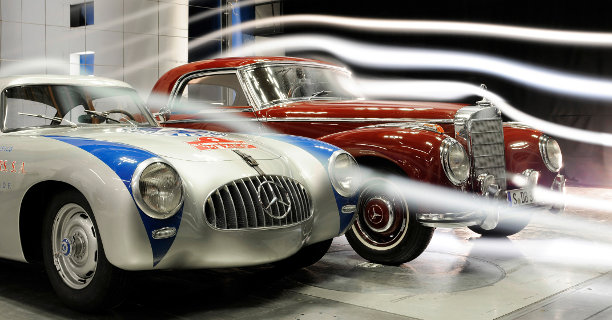
\includegraphics[width=0.618\textwidth]{pictures/aero}}
\title{Differentialgleichungen}
\subtitle{The Core of the Whole Business}
\author{}
\date{}
\lowertitleback{
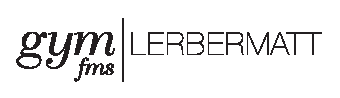
\includegraphics[height=1cm]{pictures/gymfmslerbermattlogo.eps}
\hfill%\copyright%
{\begin{tikzpicture}
  % Draw the rounded rectangle and clip the image to it
  \clip [rounded corners=5mm] (0,0) rectangle (1,1); % Adjust dimensions as needed
  \node at (0.5,0.5) {\includegraphics[width=1cm]{pictures/teacher_me_caricatur.png}}; % Adjust width and center image
\end{tikzpicture}}
}


\begin{document}
\maketitle
\tableofcontents
%\thispagestyle{empty}
\cleardoublepage
%\setcounter{page}{1}

\section{Ein erstes Beispiel}

\begin{wrapfigure}{r}{0.382\textwidth}
\vspace{-0pt}
  \begin{center}
    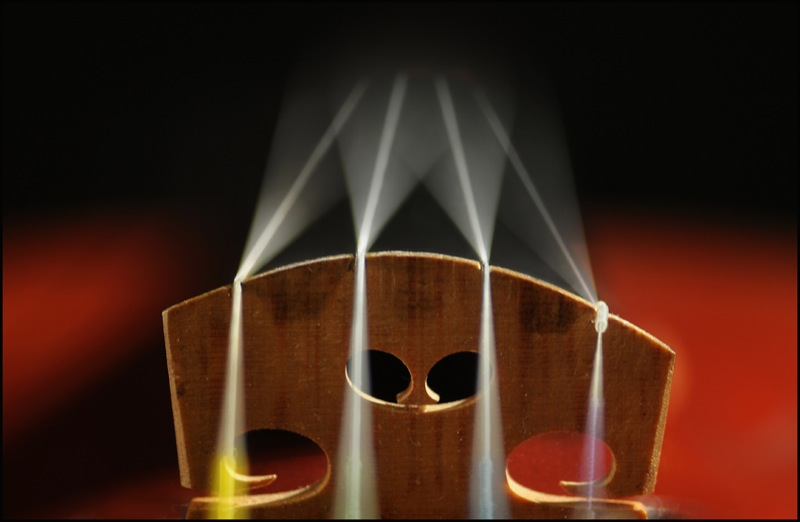
\includegraphics[width=0.37\textwidth]{pictures/geige}
  \end{center}
\caption{Geige}
\end{wrapfigure}
Wir beschäftigen uns hier mit Differentialgleichungen. Es handelt sich dabei um Gleichungen, in denen eine Funktion $f$ und Ableitungen von $f$ vorkommen. Das Interesse an Differentialgleichungen ist schon alt, denn sie eignen sich hervorragend zum Modellieren von Problemen der realen Welt, insbesondere physikalischer Natur. Die meisten Differentialgleichungen können nicht analytisch gelöst werden. Analytische Methoden liefern aber oft Aufschluss über Langzeitverhalten, Stabilität etc. Während das quantitative Verhalten heute recht bequem mit dem Computer untersucht werden kann, sind qualitative Aussagen fast ausschliesslich analytischen Untersuchungen zu verdanken.

\subsection{Problemstellung}

Als erstes, einfaches Beispiel betrachten wir die Gleichung
$$f'(x)=f(x).$$
Eine Lösung kann leicht erraten werden.

\begin{uebenv}{erstesbsp}
Nenne eine Lösungen obiger Differentialgleichung.
\end{uebenv}

\begin{cdef}[gewöhnliche Differentialgleichung]
Sucht man eine Funktion $f$ und gibt eine Relation zwischen $f$ und mindestens einer Ableitung von $f$ an, so spricht man von einer gewöhnlichen Differentialgleichung.
\end{cdef}

\subsection{Modellprobleme}

Bei einigen Problemen werde ich zur Begründung, warum gerade die angegebene Differentialgleichung untersucht wird, physikalischen Hintergrund erläutern. Diese sind aber für das Verstehen der Mathematik nicht notwendig.

\subsubsection{Der radioaktive Zerfall}

Durch
\marginnote{
\href{https://www.youtube.com/watch?v=x1g-JJ5gWuA}{\qrcode{https://www.youtube.com/watch?v=x1g-JJ5gWuA}}
}
Beobachtungen stellt man fest, dass zu einem Zeitpunkt $t$ die Anzahl Zerfälle proportional zur noch vorhandenen Stoffmenge $N(t)$ ist. Bezeichnen wir mit $N(t)$ die zum Zeitpunkt $t$ noch verbleibenden Reststoffmenge und mit $N_0$ die Stoffmenge zur Zeit $t=0$, dann haben wir

\begin{equation}\label{eq:radiozerfall}
\dot{N}(t)=-kN(t)
\end{equation}
für ein $k\in\mathbb{R}^+$. Das negative Vorzeichen in \eqref{eq:radiozerfall} interpretiert die Abnahme mit zunehmender Zeit. Wie im ersten Beispiel kann man eine Lösung sofort hinschreiben:
$$N(t)=N_0\mathrm{e}^{-kt}.$$

Wie lange dauert es, bis sich die Menge der radioaktiven Substanz halbiert hat? Bezeichnen wir mit $T$ diese \definition{Halbwertszeit}, so erhalten wir
$$T=\frac{\ln(2)}{k}$$
und stellen fest, dass $T$ unabhängig von $N_0$ ist.

\begin{uebenv}{halbwertszeit}
Leite die Formel $T=\frac{\ln(2)}{k}$ her.
\end{uebenv}

\begin{bem}
Allgemein führen Wachstums- und Zerfallsprozesse, bei denen die Veränderung proportional zur gegenwärtigen Grösse ist, auf Differentialgleichungen zu \eqref{eq:radiozerfall} ähnlicher Gestalt.
\end{bem}

\subsubsection{Das mathematische Pendel}

Ein
\marginnote{
\href{https://www.youtube.com/watch?v=Yv2XERZNB-Y}{\qrcode{https://www.youtube.com/watch?v=Yv2XERZNB-Y}}
}
Pendel der Länge $L$ und Masse $m$ sei an einem festen Punkt $P$ aufgehängt und schwinge in einer Ebene um die Ruhelage. Wir wollen den zeitlichen Verlauf dieser Bewegung studieren. Wir geben die Winkelauslenkung $\varphi$ zu jedem Zeitpunkt $t$ an, suchen also $\varphi(t)$.

\begin{figure}
\begin{center}
\begin{tikzpicture}[line cap=round,line join=round,>=triangle 45,x=1.0cm,y=1.0cm]
\clip(-4.04,-2.96) rectangle (2.86,4.46);
\draw [shift={(0,4)},color=gray,fill=gray,fill opacity=0.1] (0,0) -- (-129.12:1) arc (-129.12:-90:1) -- cycle;
\draw [shift={(0,4)}] plot[domain=4.03:5.39,variable=\t]({1*3.87*cos(\t r)+0*3.87*sin(\t r)},{0*3.87*cos(\t r)+1*3.87*sin(\t r)});
\draw (0,4)-- (0,0.13);
\draw [->] (0,4) -- (-3.88,-0.8);
\draw [->] (-2.44,1) -- (-2.44,-1.96);
\draw [->] (-2.44,1) -- (-1.1,0);
\begin{scriptsize}
\fill [color=firebrick] (-2.44,1) circle (3pt);
\draw[color=firebrick] (-2.8,1.1) node {$m$};
\draw[color=darkblue] (-1.65,2.4) node {$L$};
\draw[color=seagreen] (-0.25,3.3) node {$\varphi$};
\fill [color=lightgray] (0,4) circle (1.5pt);
\draw[color=gray] (0.25,4.2) node {$P$};
\end{scriptsize}
\end{tikzpicture}
\end{center}
\caption{Das mathematische Fadenpendel}
\end{figure}

Offensichtlich wirkt auf $m$ die Kraft $F_G=mg$, wobei der radiale Anteil dafür sorgt, dass die Schnur gespannt bleibt, und der Winkelanteil $mg\sin(\varphi)$ für die Winkelbeschleunigung $L\ddot{\varphi}$ verantwortlich ist. Damit ergibt sich
$$mL\ddot{\varphi}(t)=-mg\sin(\varphi(t)).$$
Formen wir die Gleichung nach $\ddot{\varphi}$ um und benutzen die bekannte Näherung für kleine Winkel, $\sin(\alpha)\approx\alpha$, so haben wir
\begin{equation}\label{eq:mathpendel}
\ddot{\varphi}(t)=-\frac{g}{L}\varphi(t).
\end{equation}
Setzt man
$$\omega_0=\sqrt{\frac{g}{L}}$$
ergibt sich als Lösung
$$\varphi(t)=c_1\sin(\omega_0 t)+c_2\cos(\omega_0 t),$$
wobei $c_1,c_2\in\mathbb{R}$ beliebig sind.
Man erkennt, dass für eine Anfangsauslenkung und eine Anfangsgeschwindigkeit eine eindeutige Lösung vorliegt.

\begin{uebenv}{mathpendel}
Prüfe obige Lösung in \eqref{eq:mathpendel}.
\end{uebenv}

\clearpage

\subsection{Notizen zu den Übungen}

\begin{lsg}{erstesbsp}
Beispielsweise erfüllt $f(x)=\mathrm{e}^x$ obige Differentialgleichung.
\end{lsg}
\begin{lsg}{halbwertszeit}
    Es ist $N(T)=\frac{N_0}{2}$, also $\frac{N_0}{2}=N_0\mathrm{e}^{-kT}$. Daraus folgt $\frac{1}{2}=\mathrm{e}^{-kT}$ und sofort $\ln(\frac{1}{2})=-kT\Leftrightarrow T=\frac{\ln(2)}{k}$.
\end{lsg}
\begin{lsg}{mathpendel}
    Es ist $\ddot{\varphi}(t)=-c_1\omega_0^2\sin(\omega_0 t)-c_2\omega_0^2\cos(\omega_0 t)=-\omega_0^2(c_1\sin(\omega_0 t)+c_2\cos(\omega_0 t))=-\omega_0^2\varphi(t)=-\frac{g}{L}\varphi(t)$.
\end{lsg}

\clearpage

\section{Lösungsmethoden}
\subsection{Lineare Differentialgleichungen}

\begin{cdef}[lineare Differentialgleichung]
Eine Differentialgleichung der Form

$$a_n(x)y^{(n)}(x)+a_{n-1}(x)y^{(n-1)}(x)+%\dots\\
\dots+a_0(x)y(x)=b(x)$$

heisst lineare Differentialgleichung $n$-ter Ordnung, wobei $a_n(x),\dots,a_0(x)$ und $b(x)$ Funktionen sind.
\end{cdef}

\begin{bsp}
Ein Spezialfall einer linearen Differentialgleichung zweiter Ordnung mit konstanten Koeffizienten ist
$$a_2y''(x)+a_1y'(x)+a_0y(x)=b(x).$$
Der von $x$ abhängige Ausdruck $b(x)$ wird \definition{Störterm} genannt.
\end{bsp}

\begin{cdef}[homogene und inhomogene DGL]
Ist $b(x)=0$, so heisst die Differentialgleichung homogen, andernfalls wird sie inhomogen genannt.
\end{cdef}

\begin{bem}
Für einige explizite Differentialgleichungen erster Ordnung gibt es Standardverfahren zu ihrer numerischen Lösung. Viele explizite Differentialgleichungen höherer Ordnung lassen sich in ein System von Differentialgleichungen erster Ordnung überführen, auf die dann diese Standardverfahren angewendet werden dürfen.
\end{bem}

\subsection{Separation der Variablen}

Viele Differentialgleichungen sind von der Form

$$y'=f(x)\cdot g(y).$$

Für diesen Typ lässt sich das Problem auf ein Integrationsproblem zurückführen. Die Separation der Variablen geht so:
\marginnote{
\href{https://www.youtube.com/watch?v=x1g-JJ5gWuA}{\qrcode{https://www.youtube.com/watch?v=x1g-JJ5gWuA}}
}
Man schreibt $y'$ als Quotient der Differentiale $\mathrm{d}y/\mathrm{d}x$
$$\frac{\mathrm{d}y}{\mathrm{d}x}=f(x)\cdot g(y)$$
und trennt dann die Variablen:
$$\frac{1}{g(y)}\,\mathrm{d}y=f(x)\,\mathrm{d}x.$$
Durch Integration beider Seiten erhält man die Lösungen der Differentialgleichung, nämlich
$$\int\frac{1}{g(y)}\,\mathrm{d}y=\int f(x)\,\mathrm{d}x.$$

Seien $I\subset\mathbb{R}$ ein offenes Intervall und $a,s:I\longrightarrow\mathbb{R}$ stetige Funktionen. Wir studieren die Differentialgleichungen
\begin{align}
y'(x) &= ay(x)\\
y'(x) &= ay(x)+s
\end{align}

\begin{csatz}
Die homogene lineare Differentialgleichung besitzt als Lösung genau die Funktionen $y:I\longrightarrow\mathbb{R}$ gegeben durch
$$y(x)=ce^{\int_{x_0}^xa(t)dt}$$
mit $c\in\mathbb{R}$ und $x_0\in I$.
\end{csatz}

\begin{proof}
Dass die oben beschriebenen Funktionen $y$ die Gleichung erfüllen, erkennen wir durch Ableiten. Für die Eindeutigkeit brauchen wir auch ein direktes Argument. Sei $y$ wie oben und $z$ eine weitere Lösung, so ergibt sich
$$\frac{d}{\mathrm{d}x}\frac{z}{y}=\frac{z'y-zy'}{y^2}=\frac{azy-zay}{y^2}=0.$$
Also ist $\frac{z}{y}$ konstant und somit $z=cy$.
\end{proof}

\begin{uebenv}{separation}
Löse
$$y'=(x^2+1)(y-2).$$
\end{uebenv}

\begin{lsg}{separation}
    \begin{align*}
        y' &= (x^2+1)(y-2)\\
        \frac{\mathrm{d}y}{\mathrm{d}x} &= (x^2+1)(y-2)\\
        \frac{1}{y-2}\cdot\mathrm{d}y &= (x^2+1)\cdot\mathrm{d}x\tag{$\int$}\\
        \ln(y-2) &= \frac{1}{3}x^3+x+C\tag{$\mathrm{e}^{()}$}\\
        y-2 &= \mathrm{e}^{\frac{1}{3}x^3+x+C}
    \end{align*}
    und daraus folgt die Lösung $y(x)=y_0\mathrm{e}^{\frac{1}{3}x^3+x}+2$
\end{lsg}

\begin{uebenv}{moreseparation}
Löse mit der Methode der Trennung der Variablen
\begin{enumerate}[a)]
\item $\dot{N}=-\lambda N$
\item $u'=-\frac{x^2}{u^3}$
\item $u'=u^2+1$
\item $u'=\mathrm{e}^u\sin(x)$
\end{enumerate}
\end{uebenv}

\subsection{Variation der Konstanten}

Die lineare Differentialgleichung erster Ordnung,
$$y'+g(x)y=s(x),$$
wobei $s(x)$ eine sogenannte Störfunktion ist, wird in zwei Schritten gelöst.

\begin{enumerate}
\item Man löst die zugehörige homogene Differentialgleichung
$$y' = g(x)y$$
durch Separation der Variablen.

\begin{align*}
\int\frac{\mathrm{d}y}{y} &= -\int g(x)\mathrm{d}x\\
\ln|y| &= -\int g(x)\mathrm{d}x\\
y &= ce^{-\int g(x)\mathrm{d}x}
\end{align*}
mit $c\in\mathbb{R}$.
\item Die
\marginnote{
\href{https://www.youtube.com/watch?v=uSb8s91nv_s}{\qrcode{https://www.youtube.com/watch?v=uSb8s91nv_s}}
}
Integrationskonstante $c$ wird als Funktion von $x$ angesetzt --- Variation der Konstanten.
$$y=c(x)e^{-\int g(x)\mathrm{d}x}.$$
Für die Ableitung erhalten wir
$$y' = c'(x)e^{-\int g(x)\mathrm{d}x}+c(x)(-g(x))e^{-\int g(x)\mathrm{d}x}$$
was
$$s(x)-g(x)y$$
entsprechen soll. Daraus folgt
$$c'(x)=s(x)e^{\int g(x)\mathrm{d}x}$$
also
$$c(x)=\int s(x)e^{\int g(x)\mathrm{d}x}\mathrm{d}x+K$$
Die Lösung lautet
$$y=e^{-\int g(x)\mathrm{d}x}\cdot\left(\int s(x)e^{\int g(x)\mathrm{d}x}\mathrm{d}x+K\right).$$
\end{enumerate}

\begin{csatz}
    Die allgemeine Lösung einer inhomogenen Differentialgleichung
    $$y'(x)=g(x)y(x)+s(x)$$
    erhält man, indem zur allgemeinen Lösung der zugehörigen homogenen Differentialgleichung $y'(x)=g(x)y(x)$ eine partikuläre Lösung $y_p(x)$ der inhomogenen Differentialgleichung $y'(x)=g(x)y(x)+s(x)$ addiert wird.
\end{csatz}

\begin{proof}
    Seien $y_h$ bzw. $y_p$ die allgemeine homogene bzw. eine partikuläre Lösung von $y'=gy+s$ und $y=y_h+y_p$.

    Betrachte $y_h'=y'-y_p'=gy+s-(gy_p+s)=g(y_h+y_p)+s-gy_p-s=gy_h$, also löst $y_h$ die zugehörige homogene Differentialgleichung.

    Ferner $y'=y_h'+y_p'=gy_h+gy_p+s=g(y_h+y_p)+s=gy+s$. Das heisst, dieser Ansatz erfüllt die gegebene Differentialgleichung.
\end{proof}

\begin{uebenv}{variationderkonstanten}
Löse
$$y'(x)=y(x)+x$$
\end{uebenv}

\begin{uebenv}{variationderkonstantenx}
Löse
$$y'(x)=xy(x)+x$$
\end{uebenv}

\begin{uebenv}{variationsinx}
Löse
$$y'-y\tan(x)=-\sin(x).$$
\end{uebenv}

\begin{uebenv}{variationpoly}
Löse
$$y'+\frac{y}{x}=x^2+4$$
\end{uebenv}

\begin{uebenv}{variationopenended}
Löse
$$y'(x)=\frac{1}{x^2}\cdot y(x)+\sin(x)$$
\end{uebenv}

\subsection{Exakte Gleichungen}

\begin{cdef}[Exakte Differentialgleichung]
Sei
\marginnote{
\href{https://www.youtube.com/watch?v=haiyzr8B7_A}{\qrcode{https://www.youtube.com/watch?v=haiyzr8B7_A}}
}
$\mathbb{G}\subset\mathbb{R}^n$ ein Gebiet. Die Differentialgleichung
$$P\mathrm{d}x+Q\mathrm{d}y=0$$
mit $P,Q:\mathbb{G}\longrightarrow\mathbb{R}$ heisst exakt, wenn es eine stetig differenzierbare Funktion $F:\mathbb{G}\longrightarrow\mathbb{R}$ gibt, so dass $P=\frac{\partial F}{\partial x}=F_x$ und $Q=\frac{\partial F}{\partial y}=F_y$ gilt.
\end{cdef}

Wir erhalten die Lösungen, indem wir die Niveaulinien $F^{-1}(c)$ mit $c\in\mathbb{R}$ nach einer der Variablen auflösen.

\begin{bem}
Eine Lösung $F$ der obigen DGL heisst \definition{Potentialfunktion} des Vektorfeldes $(P|Q)$.
\end{bem}

\begin{csatz}[Integrabilitätsbedingung]
    Gilt $\frac{\partial}{\partial y}P=\frac{\partial}{\partial x}Q$, dann ist die Differentialgleichung $P\mathrm{d}x+Q\mathrm{d}y=0$ exakt.
\end{csatz}

\begin{proof}
    Nach Definition einer exakten Differentialgleichung gilt für das Potential $F$: $P=\frac{\partial}{\partial x}F$ und $Q=\frac{\partial}{\partial y}F$. Daraus folgt $\frac{\partial}{\partial y}P=\frac{\partial^2}{\partial y\partial x}F$ und $\frac{\partial}{\partial x}Q=\frac{\partial^2}{\partial x\partial y}F$. Mit dem Satz von Schwarz folgt die Behauptung.
\end{proof}

Nun setzen wir voraus, dass $\mathbb{G}\subset\mathbb{R}^2$ ein Gebiet ist, und $P:\mathbb{G}\longrightarrow\mathbb{R}$, $Q:\mathbb{G}\longrightarrow\mathbb{R}$ Funktionen sind. Wenn nun die  Differentialgleichung
\begin{equation}\label{eq:exakt2}
P\mathrm{d}x+Q\mathrm{d}y=0
\end{equation}
nicht exakt ist, kann man versuchen, eine nichttriviale Funktion $M:\mathbb{G}\longrightarrow\mathbb{R}$ so zu bestimmen, dass
$$(MP)\mathrm{d}x+(MQ)\mathrm{d}y=0$$
exakt ist. Eine solche Funktion nennen wir einen \definition{integrierenden Faktor} für \eqref{eq:exakt2}. Die Lösung dieser Differentialgleichung ist auch Lösung der ursprünglichen, nicht exakten Differentialgleichung.

\begin{uebenv}{exaktedglcos}
Prüfe, ob die Differentialgleichung
$$(\cos(y)+2xy)\mathrm{d}x+(x^2-y-x\sin(y))\mathrm{d}y=0$$
exakt ist und löse, wenn möglich, in expliziter Form. Falls du nicht nach $y$ auflösen kannst, löse nach $x$.
\end{uebenv}

\begin{uebenv}{exaktedgls}
Man
\marginnote{
\href{https://www.youtube.com/watch?v=vaO64RJqjAk}{\qrcode{https://www.youtube.com/watch?v=vaO64RJqjAk}}
}
überprüfe die folgenden Gleichungen auf Exaktheit. Falls nicht Exaktheit vorliegt, versuche einen integrierenden Faktor zu finden und bestimme die Lösungen.
\begin{enumerate}[a)]
\item $yy'=x$
\item $xy'=-y$
\item $x-y+(1-x)y'=0$
\item $4x+3y^2+2xyy'=0$
\item $xy^2+y-xy'=0$
\end{enumerate}
\end{uebenv}

\subsection{Potenzreihenansatz}

Ohne ins Detail zu gehen akzeptieren wir folgenden
\begin{csatz}
Wenn
\marginnote{
\href{https://www.youtube.com/watch?v=vkUnoLXzdvc}{\qrcode{https://www.youtube.com/watch?v=vkUnoLXzdvc}}
}
die Koeffizienten einer Differentialgleichung Potenzreihen sind, dann auch die Lösungen. Die Lösungen haben zudem den gleichen Definitionsbereich wie die Koeffizientenreihen.
\end{csatz}

\begin{bsp}
    Betrachte die Differentialgleichung
    $$m\ddot{y}=-ky.$$
    Wir suchen eine Lösung $y(t)$, indem wir voraussetzen, dass ein Potenzreihenansatz
    $$y(t)=\sum_{k=0}^\infty a_kt^k$$
    obige Differentialgleichung löst.

    Wir leiten 2 Mal ab und setzen den Ansatz ein:
    $$\ddot{y}(t)=\sum_{k=2}^\infty k(k-1)a_kt^{k-2}$$
    und folglich
    $$2a_2+6a_3t+12a_4t^2+\dots = -\frac{k}{m}(a_0+a_1t+a_2t^2+\dots).$$
    Nun führen wir einen Koeffizientenvergleich durch:

    \begin{align*}
        2a_2 &= -\frac{k}{m}a_0\\
        6a_3 &= -\frac{k}{m}a_1\\
        12a_4 &= -\frac{k}{m}a_2\\
        24a_5 &= -\frac{k}{m}a_3\\
        \vdots &= \vdots
    \end{align*}

    Es folgt

    \begin{align*}
        a_2 &= -\frac{k}{2m}a_0\\
        a_3 &= -\frac{k}{6m}a_1\\
        a_4 &= -\frac{k}{12m}a_2 = (\frac{k^2}{24m^2})a_0\\
        a_5 &= -\frac{k}{20m}a_3 = (\frac{k^2}{120m^2})a_1\\
        \vdots &= \vdots
    \end{align*}

    Also haben wir als Lösung
    $$y(t)=a_0+a_1t-\frac{k}{m}\frac{a_0}{2}t^2-\frac{k}{m}\frac{a_1}{6}t^3+(\frac{k}{m})^2\frac{a_0}{24}t^4+(\frac{k}{m})^2\frac{a_1}{120}t^5+\dots$$

    Wer sich zurück an Taylorreihen erinnert sieht, dass

    $$y(t)=a_0-\frac{k}{m}\frac{a_0}{2}t^2+(\frac{k}{m})^2\frac{a_0}{24}t^4+\dots+a_1t-\frac{k}{m}\frac{a_1}{6}t^3+(\frac{k}{m})^2\frac{a_1}{120}t^5-\dots$$
    wie erwartet die bekannte Taylorreihe
    $$y(t)=a_0\cos(\omega_0t)+\frac{a_1}{\omega_0}
    \sin(\omega_0t)$$

    ist.
\end{bsp}

\begin{uebenv}{potreihe}
    Löse mit einem Potenzreihenansatz:

    \begin{enumerate}[a)]
        \item $\dot{x}=v$
        \item $\ddot{x}=a$
    \end{enumerate}
\end{uebenv}

\begin{uebenv}{potenzreiheexp}
    Löse $\dot{N}=\lambda N$ mit einem Potenzreihenansatz.
\end{uebenv}

\begin{uebenv}{potenzreiheprod}
    Löse $y\cdot y'=x$ mit einem Potenzreihenansatz.
\end{uebenv}

\begin{uebenv}{potenzreihetaylor}
Löse folgende Differentialgleichungen mit einem Potenzreihenansatz unter der Annahme, dass $x(t)$ bzw. $y(x)$ als Taylorreihe darstellbar ist.
\begin{enumerate}[a)]
\item $\dot{x}=\alpha x$
\item $\dot{x}=k\sqrt{x}$
\item $y''=\frac{6y-2}{x^2}+6x^2$
\item $y=xy'-x^2$ mit $y_0=0$
\end{enumerate}
\end{uebenv}

\clearpage

\subsection{Notizen zu den Übungen}

\begin{lsg}{separation}
    \begin{align*}
        y' &= (x^2+1)(y-2)\\
        \frac{\mathrm{d}y}{\mathrm{d}x} &= (x^2+1)(y-2)\\
        \frac{1}{y-2}\cdot\mathrm{d}y &= (x^2+1)\cdot\mathrm{d}x\tag{$\int$}\\
        \ln(y-2) &= \frac{1}{3}x^3+x+C\tag{$\mathrm{e}^{()}$}\\
        y-2 &= \mathrm{e}^{\frac{1}{3}x^3+x+C}
    \end{align*}
    und daraus folgt die Lösung $y(x)=y_0\mathrm{e}^{\frac{1}{3}x^3+x}+2$
\end{lsg}
\begin{lsg}{moreseparation}
    \begin{enumerate}[a)]
        \item \begin{align*}
            \dot{N} &= -\lambda N\\
            \frac{\mathrm{d}N}{\mathrm{d}t} &= -\lambda N\\
            \frac{1}{N}\mathrm{d}N &= -\lambda\mathrm{d}t\\
            \ln(N) &= -\lambda t+C\\
            N(t) &= N_0\mathrm{e}^{-\lambda t}
        \end{align*}
        \item \begin{align*}
            \frac{\mathrm{d}u}{\mathrm{d}x} &= \frac{-x^2}{u^3}\\
             u^3\mathrm{d}u &= -x^2\mathrm{d}x\\
             \frac{1}{4}u^4 &= -\frac{1}{3}x^3+C\\
             u(x) &= \sqrt[4]{-\frac{4}{3}x^3+4C}
        \end{align*}
        \item \begin{align*}
            \frac{\mathrm{d}u}{\mathrm{d}x} &= u^2+1\\
            \frac{1}{u^2+1}\mathrm{d}u &= \mathrm{d}x\\
            \arctan(u) &= x+C\\
            u(x) &= \tan(x+C)
        \end{align*}
        Hier stellt sich die Frage, wie man $\int\frac{1}{u^2+1}\mathrm{d}u$ bestimmt. Betrachte hierzu $\tan(\arctan(x))=x$, leite auf beiden Seiten ab und löse nach $\arctan'(x)$.
        \item \begin{align*}
            \frac{\mathrm{d}u}{\mathrm{d}x} &= \mathrm{e}^{u}\sin(x)\\
            \mathrm{e}^{-u}\mathrm{d}u &= \sin(x)\mathrm{d}x\\
            -\mathrm{e}^{-u} &= -\cos(x)+C\\
            -u &= \ln(\cos(x)-C)\\
            u(x) &= -\ln(\cos(x)-C)
        \end{align*}
    \end{enumerate}
\end{lsg}
\begin{lsg}{variationderkonstanten}
    Die homogene Lösung rechnet man selber nach und findet $y_h(x)=y_0\mathrm{e}^{x}$. Nun variieren wir die Konstante, um eine partikuläre Lösung zu finden: $y_p(x)=y_0(x)\mathrm{e}^{x}$. Mit diesem Ansatz folgt $y_p'(x)=y_0'(x)\mathrm{e}^{x}+y_0(x)\mathrm{e}^{x}$, was wir einsetzen:

    \begin{align*}
        y_0'(x)\mathrm{e}^{x}+y_0(x)\mathrm{e}^{x} &= y_0(x)\mathrm{e}^{x} + x\\
        y_0'(x)\mathrm{e}^{x} &= x\\
        y_0'(x) &= x\mathrm{e}^{-x}\\
        y_0 &= -\mathrm{e}^{-x}(x+1)
    \end{align*}
    Im Ansatz verbucht erhalten wir die partikuläre Lösung $y_p(x)=-\mathrm{e}^{-x}(x+1)\mathrm{e}^{x}=-x-1$. Damit
    $$y(x)=y_0\mathrm{e}^{x}-x-1$$
\end{lsg}
\begin{lsg}{variationderkonstantenx}
Die zugehörige homogene DGL ist

\begin{align*}
    \frac{\mathrm{d}y}{\mathrm{d}x} &= xy\\
    \frac{1}{y}\mathrm{d}y &= x\mathrm{d}x\\
    \ln(y) &= \frac{1}{2}x^2+C\\
    y_h(x) &= y_0\mathrm{e}^{\frac{1}{2}x^2}
\end{align*}

und nun variieren wir die Konstante: $y_p(x) = y_0(x)\mathrm{e}^{\frac{1}{2}x^2}$. Es ist $y_h'(x) = y_0'(x)\mathrm{e}^{\frac{1}{2}x^2}+y_0(x)\mathrm{e}^{\frac{1}{2}x^2}\cdot x$, was wir einsetzen:

\begin{align*}
    y_0'(x)\mathrm{e}^{\frac{1}{2}x^2}+y_0(x)\mathrm{e}^{\frac{1}{2}x^2}\cdot x &= xy_0(x)\mathrm{e}^{\frac{1}{2}x^2}+x\\
    y_0'(x)\mathrm{e}^{\frac{1}{2}x^2} &= x\\
    y_0'(x) &= x\mathrm{e}^{-\frac{1}{2}x^2}\\
    y_0(x) &= -\mathrm{e}^{-\frac{1}{2}x^2}
\end{align*}

Im Ansatz verwertet: $y_p(x) = y_0(x)\mathrm{e}^{\frac{1}{2}x^2} = -\mathrm{e}^{-\frac{1}{2}x^2}\mathrm{e}^{\frac{1}{2}x^2}=-1$.

Also gilt für die allgemeine Lösung der zu lösenden DGL
$$y(x) = y_0\mathrm{e}^{\frac{1}{2}x^2} - 1.$$
\end{lsg}
\begin{lsg}{variationsinx}
Zuerst die zugehörige homogene DGL:
    \begin{align*}
        y' &= y\tan(x)\\
        \frac{1}{y}\mathrm{d}y &= \tan(x)\mathrm{d}x\\
        \ln(y) &= -\ln(\cos(x))+C\\
        y_h(x) &= y_0\frac{1}{\cos(x)}
    \end{align*}
    Partikuläre Lösung mit $y_p' = y_0'\frac{1}{\cos(x)}+y_0(-\frac{1}{\cos^2(x)})\cdot(-\sin(x))$
    \begin{align*}
        y_0'\frac{1}{\cos(x)}+y_0\frac{1}{\cos^2(x)}\cdot\sin(x) &= y_0\frac{1}{\cos(x)}\tan(x)-\sin(x)\\
        y_0'\frac{1}{\cos(x)} &= -\sin(x)\\
        y_0' &= -\sin(x)\cos(x)\\
        y_0 &= \frac{1}{2}\cos^2(x)
    \end{align*}
    und eingesetzt $y_p=\frac{1}{2}\cos^2(x)\frac{1}{\cos(x)}=\frac{1}{2}{\cos(x)}$.

    Somit $y(x)=y_0\frac{1}{\cos(x)}+\frac{1}{2}{\cos(x)}$
\end{lsg}
\begin{lsg}{variationpoly}
    Homogen:

    \begin{align*}
        \frac{1}{y}\mathrm{d}y &= -\frac{1}{x}\mathrm{d}x\\
        \ln(y) &= \ln(x) +C\\
        y_h(x) = y_0\frac{1}{x}
    \end{align*}

    Partikulär, $y_p' = y_0'\frac{1}{x}+y_0(-\frac{1}{x^2})$:

    \begin{align*}
        y_0'\frac{1}{x}+y_0(-\frac{1}{x^2}) &= -\frac{y_0\frac{1}{x}}{x}+x^2+4\\
        y_0'\frac{1}{x} &= x^2+4\\
        y_0' &= x^3+4x\\
        y_0 &= \frac{1}{4}x^4+2x^2
    \end{align*}

    und daraus $y_p(x)=(\frac{1}{4}x^4+2x^2)\frac{1}{x}=\frac{1}{4}x^3+2x$.

    Schliesslich $y(x)=y_0\frac{1}{x}+\frac{1}{4}x^3+2x$
\end{lsg}
\begin{lsg}{variationopenended}
Als homogene Lösung finde ich $y_h(x)=y_0\mathrm{e}^{-\frac{1}{x}}$. Bei der Variation verwende ich den geschlossenen Ausdruck $y_0=\int \mathrm{e}^{\frac{1}{x}}\sin(x)\mathrm{d}x$. Als Lösung gebe ich bloss
$$y(x)=y_0\mathrm{e}^{-\frac{1}{x}}+\int \mathrm{e}^{\frac{1}{x}}\sin(x)\mathrm{d}x\cdot\mathrm{e}^{\frac{1}{x}}$$
\end{lsg}
\begin{lsg}{exaktedglcos}
    Es ist $\frac{\partial P}{\partial y} = -\sin(y)+2x$ und $\frac{\partial Q}{\partial x} = 2x-\sin(y)$, also ist die Integrabilitätsbedingung erfüllt und die Differentialgleichung damit exakt.

    Man bildet
    \begin{align*}
        \int (\cos(y)+2xy)\mathrm{d}x &= x\cos(y)+x^2y+C_1(y)\\
        \int (x^2-y-x\sin(y))\mathrm{d}y &= x^2y-\frac{1}{2}y^2+x\cos(y)+C_2(x)
    \end{align*}
    und erkennt $F(x,y)=x^2y-\frac{1}{2}y^2+x\cos(y)$. Die Niveaulinien erhalten wir aus $x^2y-\frac{1}{2}y^2+x\cos(y)\stackrel{!}{=}k$. Diese Gleichung lösen wir vorzugsweise nach $x$:
    $$x_{1,2}=\frac{-\cos(y)\pm\sqrt{\cos^2(y)+2y^3+4yk}}{2y}$$

    \begin{figure}[h]
    \centering
    \begin{tikzpicture}
\begin{axis}[
  	%hide axis,
	xlabel=$x$,ylabel=$y$,
	mesh/interior colormap name=hot,
	colormap/blackwhite,
 ]
  \addplot3[domain=-4:4,surf,samples=10]
  	{x^2*y-1/2*y^2+x*cos(y)};
\end{axis}
\end{tikzpicture}
    \caption{Potential $F(x,y)=x^2y-\frac{1}{2}y^2+x\cos(y)$}
\end{figure}
\end{lsg}
\begin{lsg}{exaktedgls}
    \begin{enumerate}[a)]
        \item Umgeschrieben $-x\mathrm{d}x+y\mathrm{d}y=0$. Die DGL ist exakt.

        \begin{align*}
            \int (-x)\mathrm{d}x &= -\frac{1}{2}x^2+C_1(y)\\
            \int y\mathrm{d}y &= \frac{1}{2}y^2+C_2(x)
        \end{align*}
        ergibt $F(x,y)=\frac{1}{2}y^2-\frac{1}{2}x^2$ und für die Niveaulinien $y(x)=\pm\sqrt{x^2+2k}$

        \begin{figure}[h!]
    \centering
    \begin{tikzpicture}
\begin{axis}[
  	%hide axis,
	xlabel=$x$,ylabel=$y$,
	mesh/interior colormap name=hot,
	colormap/blackwhite,
 ]
  \addplot3[domain=-4:4,surf,samples=10]
  	{-0.5*x^2+0.5*y^2};
\end{axis}
\end{tikzpicture}
    \caption{Potential $F(x,y)=-0.5x^2+0.5y^2$}
\end{figure}

        \item Umgeschrieben $y\mathrm{d}x+x\mathrm{d}y=0$. Die DGL ist exakt.

        \begin{align*}
            \int y\mathrm{d}x &= xy+C_1(y)\\
            \int x\mathrm{d}y &= xy+C_2(x)
        \end{align*}
        ergibt $F(x,y)=xy$ und für die Niveaulinien $y(x)=\frac{k}{x}$

        \begin{figure}[h!]
    \centering
    \begin{tikzpicture}
\begin{axis}[
  	%hide axis,
  	%grid=both,
	xlabel=$x$,ylabel=$y$,
	mesh/interior colormap name=hot,
	colormap/blackwhite, 
 ]
  \addplot3[domain=-4:4,surf,samples=10]
  	{x*y};
\end{axis}
\end{tikzpicture}
    \caption{Potential $F(x,y)=xy$}
    \label{fig:potxy}
\end{figure}

        \item Umgeschrieben $(x-y)\mathrm{d}x+(1-x)\mathrm{d}y=0$. Die DGL ist exakt.

        \begin{align*}
            \int (x-y)\mathrm{d}x &= \frac{1}{2}x^2-xy+C_1(y)\\
            \int (1-x)\mathrm{d}y &= y-xy+C_2(x)
        \end{align*}
        ergibt $F(x,y)=\frac{1}{2}x^2+y-xy$ und für die Niveaulinien $y(x)=\frac{-\frac{1}{2}x^2+k}{1-x}$

        \begin{figure}[h!]
    \centering
    \begin{tikzpicture}
\begin{axis}[
  	%hide axis,
  	%grid=both,
	xlabel=$x$,ylabel=$y$,
	mesh/interior colormap name=hot,
	colormap/blackwhite, 
 ]
  \addplot3[domain=-4:4,surf,samples=10]
  	{0.5*x^2-x*y+y};
\end{axis}
\end{tikzpicture}
    \caption{Potential $F(x,y)=0.5x^2-xy+y$}
    \label{fig:potxyundy}
\end{figure}

        \item Umgeschrieben $(4x+3y^2)\mathrm{d}x+2xy\mathrm{d}y=0$. Die DGL ist nicht exakt. Man findet als integrierenden Faktor $M(x,y)=x^2$.

        \begin{align*}
            \int (4x^3+3y^2x^2)\mathrm{d}x &= x^4+y^2x^3+C_1(y)\\
            \int 2x^3y\mathrm{d}y &= x^3y^2+C_2(x)
        \end{align*}
        ergibt $F(x,y)=x^4+y^2x^3$ und für die Niveaulinien $y(x)=\pm\sqrt{\frac{-x^4+k}{x^3}}$.

        \begin{figure}[h!]
    \centering
    \begin{tikzpicture}
\begin{axis}[
  	%hide axis,
  	%grid=both,
	xlabel=$x$,ylabel=$y$,
	mesh/interior colormap name=hot,
	colormap/blackwhite, 
 ]
  \addplot3[domain=-2:2,surf,samples=20]
  	{x^4-x^3*y^2};
\end{axis}
\end{tikzpicture}
    \caption{Potential $F(x,y)=x^4+x^3y^2$}
\end{figure}

        \item Umgeschrieben $(xy^2+y)\mathrm{d}x-x\mathrm{d}y=0$. Die DGL ist nicht exakt. Man findet als integrierenden Faktor $M(x,y)=\frac{1}{y^2}$

        \begin{align*}
            \int (x+\frac{1}{y})\mathrm{d}x &= \frac{1}{2}x^2+\frac{x}{y}+C_1(y)\\
            \int (-\frac{x}{y^2})\mathrm{d}y &= \frac{x}{y}+C_2(x)
        \end{align*}
        ergibt $F(x,y)=\frac{1}{2}x^2+\frac{x}{y}$ und für die Niveaulinien $y(x)=-\frac{2x}{x^2+k}$.

        \begin{figure}[h!]
    \centering
    \begin{tikzpicture}
\begin{axis}[
  	%hide axis,
  	grid=both,
	xlabel=$x$,ylabel=$y$,
	mesh/interior colormap name=hot,
	colormap/blackwhite,
	restrict z to domain=-10:10,
 ]
  \addplot3[domain=-2:2,surf, samples=20
  %point meta={0.5*x^2+x/y>10 ? nan : z},
  ]
  {0.5*x^2+x/y};
\end{axis}
\end{tikzpicture}
    \caption{Potential $F(x,y)=0.5x^2+\frac{x}{y}$}
\end{figure}
    \end{enumerate}
\end{lsg}
\begin{lsg}{potreihe}
    \begin{enumerate}[a)]
        \item Mit dem Ansatz $x(t)=\sum_{k=0}^\infty a_kt^k$ ist die erste Ableitung $\dot{x}(t)=\sum_{k=1}^\infty ka_kt^{k-1}$. Eingesetzt sehen wir
        $$a_1+2a_2t+3a_3t^2+\dots = v$$
        und daraus $a_1=v$ und $a_k=0$ für $k\geq2$. Somit ist die Lösung $x(t)=a_0+vt$
        \item Wir verwenden von oben $\dot{x}$ und leiten ein weiteres Mal ab: $\ddot{x}=\sum_{k=2}^\infty k(k-1)a_kt^{k-2}$. Es folgt
        $$2a_2+6a_3t+12a_4t^2+\dots = a$$
        und $a_2=\frac{1}{2}a$ sowie $a_k=0$ für $k\geq3$. Die Lösung ist also $x(t)=a_0+a_1t+\frac{1}{2}at^2$
        
    \end{enumerate}
\end{lsg}
\begin{lsg}{potenzreiheexp}
    Setze $N(t)=a_0+a_1t+a_2t^2+\dots$. Somit $\dot{N}=a_1+2a_2t+3a_3t^2+\dots$. Der Koeffizientenvergleich ergibt $a_1=\lambda a_0$ und weiter
    \begin{align*}
        a_2 &= \frac{\lambda}{2}a_1=\frac{\lambda^2}{2}a_0\\
        a_3 &= \frac{\lambda}{3}a_2=\frac{\lambda^3}{6}a_0\\
        a_4 &= \frac{\lambda}{4}a_3=\frac{\lambda^4}{24}a_0\\
        \vdots &= \vdots
    \end{align*}
    Die Lösung ist wie erwartet
    $$N(t)=a_0+\lambda a_0t+\frac{\lambda^2}{2}a_0t^2+\frac{\lambda^3}{6}a_0t^3+\dots = a_0\sum_{k=0}^\infty \frac{\lambda ^k}{k!}t^k=a_0\cdot\mathrm{e}^{\lambda t}.$$
\end{lsg}
\begin{lsg}{potenzreiheprod}
    Wir nehmen den Ansatz $y(x)=a_0+a_1x+a_2x^2+\dots$ mit Ableitung $y'(x)=a_1+2a_2t+3a_3t^2+\dots$. Wenn wir die ersten paar Summanden ausmultiplizieren und einsetzen
    $$a_0a_1+(2a_0a_2+a_1^2)x+(3a_0a_3+3a_1a_2)x^2+\dots\stackrel{!}{=}x$$
    erfüllen wir alle Gleichungen, wenn $a_k=0\,(\forall k\in\mathbb{N}_0\setminus\{1\})$ ausser $a_1=1$.
\end{lsg}
\begin{lsg}{potenzreihetaylor}
    \begin{enumerate}[a)]
        \item Der abgeleitete Ansatz liefert $\dot{x}(t)=a_1+2a_2t+3a_3t^2+\dots$. Damit erhalten wir die Gleichungen $a_1=\alpha a_0$, $a_2=\frac{\alpha^2}{2!}a_0$, $a_3=\frac{\alpha^3}{3!}a_0$ bzw. $a_k=\frac{\alpha^k}{k!}$, also $x(t)=a_0(1+\alpha t+\frac{\alpha^2}{2!}t^2+\dots)=a_0\mathrm{e}^{\alpha t}$.
        \item Mit Quadrieren erhalten wir $\dot{x}^2=k^2x$ und es folgt
        $$(a_1+2a_2t+3a_3t^3+\dots)(a_1+2a_2t+3a_3t^3+\dots)=k^2(a_0+a_1t+a_2t^2+\dots).$$
        Durch Koeffizientenvergleich finden wir
        \begin{align*}
            a_1=\pm k\sqrt{a_0},\quad a_2=\frac{k^2}{4},\quad 6a_1a_3+4a_2^2 &= k^2a_2\\
            6k\sqrt{a_0}a_3+\frac{k^4}{4} &= \frac{k^4}{4}\\
            a_0=0\text{ oder } a_3 &= 0
        \end{align*}
        Für $a_0=0$ folgt $a_1=0$ und also $x(t)=\frac{k^2}{4}t^2$. Für $a_0\neq0$ würde $x(t)=a_0+k\sqrt{a_0}t+\frac{k^2}{4}t^2$ folgen, das aber einem Check nicht standhält.
        \item Nach Multiplikation mit $x^2$ lösen wir
        $$y''x^2=6y-2+6x^4.$$
        Wir haben $y''=2a_2+6a_3x+12a_4x^2$ und vergleichen die Koeffizienten in
        $$2a_2x^2+6a_3x^3+12a_4x^4+\dots=6a_0-2+6a_1x+6a_2x^2+6a_3x^3+(6a_4+6)x^4+\dots.$$
        Es folgt $a_0=\frac{1}{3}$, $a_3$ beliebig und $a_4=1$. Alle andern $a_k$ sind $0$. Somit $y(x)=\frac{1}{3}+a_3x^3+x^4$.
        \item $$a_0+a_1x+(a_2+1)x^2+a_3x+\dots=a_1x+2a_2x^2+3a_3x^3+\dots$$
        und unmittelbar $a_0=0$, $a_1$ beliebig, $a_2=1$ und alle andern $a_k=0$. Also $y(x)=a_1x+x^2$
    \end{enumerate}
\end{lsg}

\clearpage

\section{Gravitationskraft und Luftwiderstand}
\subsection{Freier Fall}

\begin{wrapfigure}{r}{0.3\textwidth}
\vspace{-35pt}
  \begin{center}
    
\includegraphics[width=0.24\textwidth]{pictures/fall}
  \end{center}
\caption{First Law of Cartoon Physics}
\vspace{-35pt}
\end{wrapfigure}

Wir betrachten die Geschwindigkeit $v$ für den freien Fall ohne Luftwiderstand unter konstanter Beschleunigung $g$,
$$\dot{v}=g.$$

\begin{bem}
In der Physik ist es üblich, die Ableitung nach der Zeit mit einem Punkt und die Ableitung nach dem Ort mit einem Strich zu bezeichnen.
\end{bem}

Durch Integrieren über die Zeit $t$ erhält man die Bewegungsgleichung Lösung zur Anfangsgeschwindigkeit $v_0$ und zum Startpunkt $s_0$, nämlich

\begin{align*}
v &= v_0+gt\\
s &= s_0+v_0t+\frac{1}{2}gt^2
\end{align*}

\begin{uebenv}{glmbeschl}
    Rechne die Ausdrücke für die Geschwindigkeit $v(t)$ und den Ort $s(t)$ nach.
\end{uebenv}

\subsection{Fall mit Luftwiderstand}

Hier setzen wir wiederum konstante Erdbeschleunigung $g$ voraus, aber berücksichtigen den Luftwiderstand, $F_R=\frac{1}{2}\rho_L c_wAv^2$, wobei $c$ konstant ist. Wir dividieren die Bewegungsgleichung $m\dot{v}=mg-\beta v^2$ durch $m$ und setzen $\alpha = \frac{\beta}{m}$:

$$
\dot{v}=g-\alpha v^2.
$$

Wir interessieren uns für die Geschwindigkeitsfunktion $v(t)$, nach der wir lösen wollen. Separation der Variablen liefert:

\begin{align*}
    \frac{1}{g-\alpha v^2}\,\mathrm{d}v &= \mathrm{d}t\\
    \frac{1}{\alpha}\cdot\frac{1}{\left(\sqrt{\frac{g}{\alpha}}\right)^2-v^2}\,\mathrm{dv} &= \mathrm{d}t
\end{align*}

Die Differenz der beiden Quadrate kann man \enquote{integrierbarer} bereitstellen, wenn man folgende Substitution vornimmt. Setze $v:=\sqrt{\frac{g}{\alpha}}\tanh(u)$ und leite ab, um $\frac{\mathrm{d}v}{\mathrm{d}u}=\sqrt{\frac{g}{\alpha}}\mathrm{sech}^2(u)$. Damit folgt

$$
\frac{\sqrt{\frac{g}{\alpha}}\cdot\mathrm{sech}^2(u)}{g-\alpha \left(\frac{g}{\alpha}\tanh^2(u)\right)}\,\mathrm{d}u = 
\frac{\sqrt{\frac{g}{\alpha}}\cdot\mathrm{sech}^2(u)}{g\cdot\mathrm{sech}^2(u)}\,\mathrm{d}u =
\frac{1}{\sqrt{g\alpha}}\,\mathrm{d}u
$$

Damit integriert erhalten wir

\begin{align*}
    \frac{1}{\sqrt{g\alpha}}\cdot u &= t+C\\
    \frac{1}{\sqrt{g\alpha}}\mathrm{artanh}\left(\frac{v}{\sqrt{\frac{g}{\alpha}}}\right) &= t+C\\
    v(t) &= \sqrt{\frac{g}{\alpha}}\tanh(\sqrt{g\alpha}(t+C)
\end{align*}

und mit $v(0)=:v_0$ folgt:

$$
v(t)=\sqrt{\frac{mg}{\beta}}\cdot\tanh\left(\sqrt{\frac{g\beta}{m}}\cdot t + \mathrm{artanh}\left(\sqrt{\frac{g\beta}{m}}\cdot v_0\right)\right)
$$

Als Lösung zur Anfangsgeschwindigkeit $v_0=0$ erhalten wir
$$v=\sqrt{\frac{mg}{\beta}}\tanh\left(\sqrt{\frac{g\beta}{m}}t\right).$$

Betrachtet man $\tanh$, so erkennt man die Maximalgeschwindigkeit
$$v_{max}=\sqrt{\frac{mg}{\beta}}.$$

\begin{uebenv}{geschwfreierfall}
    Skizziere den Geschwindigkeitsverlauf $v(t)$ in einem Koordinatensystem.
\end{uebenv}

\subsection{Freier Fall aus grosser Höhe}

Nach Newton nimmt die Gravitationskraft mit zunehmender Entfernung quadratisch ab:
$$g=-\frac{\mu}{r^2}.$$
Ohne Luftwiderstand gilt
$$\ddot{r}=-\frac{\mu}{r^2},$$
was wir auf beiden Seiten mit $\dot{r}$ multiplizieren:
$$\ddot{r}\dot{r}=-\frac{\mu\dot{r}}{r^2}.$$
Integrieren auf beiden Seiten führt uns zum Energieerhaltungssatz
$$0.5\dot{r}^2=\frac{\mu}{r}+c$$
und schliesslich zur Differentialgleichung
$$\dot{r}=\pm\sqrt{2\frac{\mu}{r}+c}.$$
Nun kann man die Variablen separieren und versuchen, die Integrale zu bestimmen.

\subsection{Barometrische Höhenformel}

Wir
\marginnote{
\href{https://www.youtube.com/watch?v=wUwE41Z-Q3U}{\qrcode{https://www.youtube.com/watch?v=wUwE41Z-Q3U}}
}
gehen von der Zustandsleichung für ideale Gase,
$$pV=nRT,$$
aus, wobei $p(h)$ den Luftdruck in der Höhe $h$, $V$ das Volumen, $n$ die Masse in Mol, $R$ die allgemeine Gaskonstante und $T$ die Temperatur bezeichnen. Die Atmosphäre sei eine ruhende Gasschicht, die sich wie ein ideales Gas verhalte.

Wir betrachten eine kleine Höhenänderung $\mathrm{d}h$ bezüglich der Querschnittsfläche $A$:
\begin{align*}
    p(h+\mathrm{d}h)-p(h) &= -\frac{mg}{A}\\
    &= -\frac{\rho A\cdot \mathrm{d}h\cdot g}{A}\\
    &= -\rho g\cdot \mathrm{d}h
\end{align*}

Die Dichte hängt ebenfalls von der Höhe ab, $\rho(h)$. Unter Benutzung der Zustandsgleichung für ideale Gase kann $\rho$ durch $p$ ersetzt werden:
$$\rho=\frac{m}{V}=\frac{mp}{nRT}=\frac{Mp}{RT}$$
wobei $M$ das Molekulargewicht der Luft bezeichnen soll. Damit folgt
$$p(h+\mathrm{d}h)-p(h)=-\frac{M}{RT}g\cdot \mathrm{d}h,$$
also
$$\frac{dp}{dh}=-\frac{Mg}{RT}\cdot p$$
Durch Integrieren erhalten wir die barometrische, isotherme Höhenformel
$$p(h)=p_0\cdot \mathrm{e}^{-\frac{Mgh}{RT}}.$$
Fassen wir die Konstanten zusammen:
$$h_0=\frac{RT}{Mg}\approx\unit[8.3]{km},$$
notiert man
$$p(h)=p_0\cdot e^{-\frac{h}{h_0}}$$
und sieht, dass der Druck alle $\unit[8.3]{km}$ um den Faktor $\mathrm{e}$ abnimmt. Da die Temperatur allerdings auch mit der Höhe abnimmt --- und nicht wie angenommen konstant bleibt --- ist dies nur eine Näherung; die Dichte muss rascher abnehmen.

Falls die Temperatur mit der Höhe linear abnimmt,
$$T(h)=T_0-\lambda(h-h_0),$$
wobei $\lambda$ den Temperaturgradienten bezeichne (ca. $6.5\,$Kelvin pro Kilometer), erhalten wir
$$p=p_0\left(\frac{T_0-\lambda(h-h_0)}{T_0}\right)^{\frac{g}{R\lambda}}.$$
Diese Form wird in der Meteorologie und Luftfahrt oft verwendet.

\begin{uebenv}{meteodruck}
    Rechne die meteorologische Höhenformel nach.
\end{uebenv}

\clearpage

\subsection{Notizen zu den Übungen}

\begin{lsg}{glmbeschl}
    Es ist
    $$v(t)=\int g\,\mathrm{d}t=gt+v_0$$
    und
    $$s(t)=\int(gt+v_0)\,\mathrm{d}t=\frac{1}{2}gt^2+v_0t+s_0.$$
\end{lsg}
\begin{lsg}{geschwfreierfall}
    Ich setze beispielsweise $m=81\,\mathrm{kg}$, $g\approx 9\,\mathrm{\frac{m}{s^2}}$, $v_0=0\,\mathrm{\frac{m}{s}}$ und $c_w=1$. Schätze nun die Querschnittsfläche $A$ und die durchschnittliche Luftdichte $\rho_L$. Damit wird $\beta\approx\frac{1}{3}$, den Graphen zeichnet man mit \geogebralink\ und die maximale Geschwindigkeit ist ungefähr $180\,\mathrm{\frac{km}{h}}$.
\end{lsg}
\begin{lsg}{meteodruck}
    Wir starten mit der hydrostatischen Gleichung
    $$\mathrm{d}p=-\frac{p}{RT}g\,\mathrm{d}h$$
    woraus
    $$\frac{\mathrm{d}p}{p}=-\frac{1}{R(T_0-\lambda(h-h_0))}g\,\mathrm{d}h$$
    folgt. Durch Integration via Separation erhalten wir
    $$\ln(p)=-\frac{g}{R\lambda}\ln(T_0-\lambda(h-h_0))+C$$
    und nach Exponentiation sowie mit der Randbedingung $p(h_0)=p_0$ schliesslich
    $$p=p_0\left(\frac{T_0-\lambda(h-h_0)}{T_0}\right)^{\frac{g}{R\lambda}}$$
    die barometrischen Höhenformel mit Temperaturgradient.
\end{lsg}

\clearpage

\section{RC-Glied}

Wir
\marginnote{
\href{https://www.youtube.com/watch?v=oLtU1l0dC9A}{\qrcode{https://www.youtube.com/watch?v=oLtU1l0dC9A}}
}
verwenden das bekannte
$$U=RI=\frac{Q}{C}.$$
Da der Strom die Änderung der Ladung pro Zeit darstellt, $\dot{Q}=-I$, folgt
$$\dot{Q}=-\frac{Q}{RC}.$$

Als Lösung mit $Q(0)=Q_0$ erhält man  
$$Q=Q_0 \mathrm{e}^{-\frac{t}{RC}}.$$

\begin{uebenv}{circuit}
    Rechne die Lösung nach.
\end{uebenv}

\begin{figure}[h!]
\begin{center}
    \begin{circuitikz}
        \draw
        (0,0) to[sinusoidal voltage source, l=$U_s$] (0,2) 
        to[closing switch, l=$S$] (1.5,2) % Schalter
        to[R, european, l=$R$] (3,2) 
        to[C, l=$C$] (6,2) 
        to[short] (6,0) -- (0,0);
    \end{circuitikz}
\end{center}
\caption{Schema des Stromkreises}\label{abb:stromkreis}
\end{figure}

\clearpage

\subsection{Notizen zu den Übungen}

\begin{lsg}{circuit}
    Es ist
    \begin{align*}
        \dot{Q} &= -\frac{1}{RC}Q\tag{$\cdot\mathrm{d}t$}\\
        \mathrm{d}Q &= -\frac{1}{RC}Q\,\mathrm{d}t\\
        \frac{1}{Q}\,\mathrm{d}Q &= -\frac{1}{RC}\,\mathrm{d}t\tag{$\int$}\\
        \ln(Q) &= -\frac{1}{RC}t+C\\
        Q &= \mathrm{e}^{-\frac{1}{RC}t+C}\\
        Q(t) &= Q_0\mathrm{e}^{-\frac{1}{RC}t}\\
    \end{align*}
\end{lsg}

\clearpage

\section{Taylor-Reihe}
\begin{figure}
  \begin{center}
    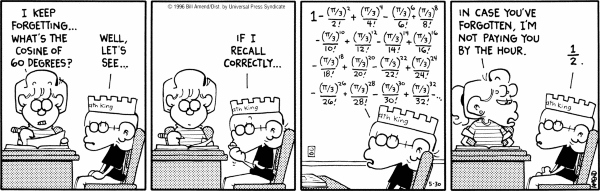
\includegraphics[width=0.618\textwidth]{pictures/taylor}
  \end{center}
\caption{MacLaurin-Reihe von $\cos(x)$}
\end{figure}

\begin{uebenv}{taylorpoly}
    Betrachte das Polynom $n$-ten Grades
    $$f(x)=a_nx^n+a_{n-1}x^{n-1}+\dots+a_1x+a_0.$$
    Notiere $f^{(k)}(0)$ für $k\in\{0,\dots,n\}$.
\end{uebenv}

Daraus schliesst man, dass die Funktion $f$ in der Form
$$f(x)=\frac{f^{(n)}(0)}{n!}x^n+\frac{f^{(n-1)}(0)}{(n-1)!}x^{n-1}+\dots+\frac{f'(0)}{1!}x+f(0)$$
dargestellt werden kann.
Da viele Funktionen näherungsweise als Reihe dargestellt werden können, definiert man

\begin{cdef}[MacLaurin-Reihe]
Sei $f$ eine bei $x=0$ definierte und beliebig oft differenzierbare Funktion. Dann heisst das Polynom
$$\mathcal{T}f(x)_{x_0=0}=f(0)+\frac{f'(0)}{1!}x+\frac{f''(0)}{2!}x^2+\frac{f'''(0)}{3!}x^3+\dots$$
MacLaurin-Reihe.
Soll
\marginnote{
\href{https://www.youtube.com/watch?v=C5s-wQSWggY}{\qrcode{https://www.youtube.com/watch?v=C5s-wQSWggY}}
}
nicht zwangsläufig um $x=0$ entwickelt werden, so spricht man allgemein von einer \definition{Taylor-Reihe}.
\end{cdef}

\begin{bsp}
Wir betrachten einige Funktionen und deren Taylorentwicklung um $x=0$.
\begin{enumerate}[a)]
\item Für $\sin(x)$ erhalten wir die bereits bekannte Darstellung
$$\mathcal{T}\sin(x)_{x_0=0}=x-\frac{x^3}{3!}+\frac{x^5}{5!}-\dots.$$
Es scheint so, als ob $\sin(x)$ als Taylorreihe darstellbar wöre.
\item $f(x)=\frac{1}{1-x}$ wird zu
$$\mathcal{T}f(x)_{x_0=0}=1+x+x^2+x^3+\dots,$$
was wir aus der Theorie über Folgen \& Reihen kennen. Damit kann aber die Taylorentwicklung höchstens für $-1<x<1$ gegen $f$ konvergieren.
\item Betrachten wir $g(x)=e^{-\frac{1}{x^2}}$ für $x\neq0$ mit seiner stetigen Fortsetzung $g(0)=0$, erhalten wir
$$\mathcal{T}g(x)_{x_0=0}=0.$$
Daher wird also $f$ nur in $x=0$ durch ihre Taylorreihe approximiert.
\end{enumerate}
\end{bsp}

\begin{cdef}[analytisch]
Eine Funktion $f$ heisst analytisch, falls sie in jedem Punkt durch eine konvergente Potenzreihe dargestellt werden kann.
\end{cdef}

Zu den analytischen Funktionen gehören die Polynome, die trigonometrischen und Exponentialfunktionen und deren Umkehrfunktionen, sowie die aus ihnen durch Grundrechenarten erzeugten Funktionen.

\begin{uebenv}{taylorreihen}
    Bestimme die Taylorreihen um $x_0=0$ der folgenden Funktionen.
    \begin{enumerate}[a)]
        \item $f(x)=e^x$
        \item $f(x)=\ln(1+x)$
    \end{enumerate}
\end{uebenv}

Für die Taylorentwicklung in einem Punkt $x_0\neq0$ einer Funktion $f$ findet man
$$\mathcal{T}f(x)_{x_0}=f(x_0)+f'(x_0)(x-x_0)+\frac{f''(x_0)}{2!}(x-x_0)^2+\dots=\sum_{k=0}^\infty \frac{f^{(k)}(x_0)}{k!}(x-x_0)^k.$$

\begin{uebenv}{taylorseries}
Bestimme die Taylorentwicklung bei $x_0$ von
$$f(x)=\frac{1}{1-x}.$$
Berechne dazu zuerst $f^{(k)}(x)$. Notiere dann $\mathcal{T}f(x)_{x_0=a}$ in geschlossener Form und explizite die ersten drei Summanden. Berechne anschliessend Näherungen für z.B. $x_0=-2,0,2,\dots$.
\end{uebenv}

\subsection{Rechnen mit Potenzreihen}

Schaut man sich die ersten vier nichtverschwindenden Terme der MacLaurin-Reihe von $\sin(x^2)$ an, so stellt man sich die Frage, ob diese Funktion nicht einfacher zu entwickeln wäre.

\begin{align*}
f(x) &= \sin(x^2) \\
f'(x) &= 2x\cos(x^2) \\
f''(x) &= 2\cos(x^2)-4x^2\sin(x^2) \\
f'''(x) &= -8x^3\cos(x^2)-12x\sin(x^2) \\
f^{(4)}(x) &= 16x^4\sin(x^2)-48x^2\cos(x^2)-12\sin(x^2)
\end{align*}
Somit $T(x)=x^2+\dots$ und die weiteren Terme sind mühsam zu bestimmen. Einfacher geht es aber mit folgendem Satz.

\begin{csatz}[Konvergenzradius Taylorreihe]
Innerhalb des Konvergenzradius dürfen Potenzreihen addiert, subtrahiert, multipliziert und dividiert, gliedweise differenziert und integriert und in den Potenzreihen substituiert werden.
\end{csatz}

\begin{proof}
    Skizze: Mit dem Wurzelkriterium für Konvergenz findet man für den Radius
    $$R=\frac{1}{\lim\mathrm{sup}_{k\to\infty} |a_k|^{\frac{1}{k}}}.$$
    Daraus nimmt man immer einen lokal minimalen Wert.
\end{proof}

\begin{bsp}
$$\sin(x^2)=x^2-\frac{x^6}{3!}+\frac{x^{10}}{5!}-\frac{x^{14}}{7!}+\dots$$
\end{bsp}

\begin{bsp}
\begin{align*}
\sin x\cdot\cos x &= \left(x-\frac{x^3}{3!}+\frac{x^5}{5!}+\frac{x^7}{7!}+\dots\right)
\cdot\left(1-\frac{x^2}{2!}+\frac{x^4}{4!}-\frac{x^6}{6!}+\dots\right)\\
 &= x-\left(\frac{1}{2!1!}+\frac{1}{3!}\right)x^3+
 +\left(\frac{1}{5!}+\frac{1}{4!1!}+\frac{1}{3!2!}\right)x^5-\dots\\
 &\stackrel{*}{=}x-\frac{4}{3!}x^3+\frac{16}{5!}x^5-\frac{64}{7!}x^7+\dots\\
 &=\frac{1}{2}\left(2x-\frac{(2x)^3}{3!}+\frac{(2x)^5}{5!}-\frac{(2x)^7}{7!}+\dots\right)\\
 &=\frac{1}{2}\sin(2x)
\end{align*}
Wir begründen noch die Umformung bei $*$:
\begin{align*}
&\phantom{=}\frac{1}{(2k+1)!}+\frac{1}{(2k)!\cdot1!}+\frac{1}{(2k-1)!\cdot2!}
+\dots+\frac{1}{(k+1)!k!}\\
&=\frac{1+(2k+1)+\frac{(2k+1)2k}{2!}+\dots+\frac{(2k+1)!}{(k+1)!k!}}{(2k+1)!}\\
&=\frac{\binom{2k+1}{0}+\binom{2k+1}{1}+\dots+\binom{2k+1}{k+1}}{(2k+1)!}\\
&=\frac{2^{2k+1}/2}{(2k+1)!}\\
&=\frac{2^{2k}}{(2k+1)!}
\end{align*}
\end{bsp}

\begin{uebenv}{maclaurinreihe}
Gib die ersten $4$ nicht verschwindenden Terme der MacLaurin-Reihe für
\begin{enumerate}[a)]
\item $f(x)=\frac{x}{1-x^2}$
\item $g(x)=\frac{\ln(x+1)}{x}$
\item $h(x)=\ln(x)$
\end{enumerate}
\end{uebenv}

Ist eine Funktion $f$ durch ihre Taylorreihe darstellbar, so kann auf beiden Seiten der Gleichung abgeleitet oder integriert werden. Damit erhält man neue Beziehungen.

\begin{bsp}
Sei
$$f(x)=\frac{1}{1-x}=1+x+x^2+x^3+\dots,$$
dann folgt bei Ableitung die aus der Wahrscheinlichkeitsrechnung bekannte \glqq Warten-auf-einen-Erfolg-Wahrscheinlichkeit\grqq
$$f'(x)=\frac{1}{(1-x)^2}=1+2x+3x^2+\dots.$$
Integriert man, so erscheint
$$\int f(x) \mathrm{d}x=-\ln(1-x)=x+\frac{1}{2}x^2+\frac{1}{3}x^3+\dots.$$
\end{bsp}

\begin{bem}
Als Zückerchen erhält man Näherungen für Stammfunktionen nicht geschlossen integrierbaren Funktionen wie zum Beispiel
$$
\int e^{x^2}\mathrm{d}x =\int\left(1+x^2+\frac{x^4}{2!}+\dots\right)\mathrm{d}x=x+\frac{1}{3}x^3+\frac{1}{10}x^5+\dots.
$$
\end{bem}

Nun ist auch klar, dass sich Taylorreihen eignen, um numerische Lösungen von Differentialgleichungen zu finden. Wir verfolgen
\begin{bsp}
Betrachte
$$y''=y-x^3$$
mit den Anfangsbedingungen $f(0)=a_0=0$ und $f'(0)=a_1=6$. Wir wählen als Ansatz eine Potenzreihe
$$y=a_0+a_1x+a_2x^2+a_3x^3+\dots$$
mit zweiter Ableitung
$$y''=2a_2+6a_3x+12a_4x^2+20x^3+\dots.$$
Daraus erhalten wir
$$y-x^3=a_0+a_1x+a_2x^2+(a_3-1)x^3+\dots.$$
Es folgt
\begin{align*}
a_2&=\frac{1}{2}a_0, &a_3&=\frac{1}{6}a_1,\\
a_4&=\frac{1}{12}a_2=\frac{1}{24}a_0, &a_5&=\frac{1}{20}(\frac{1}{6}a_1-1)
\end{align*}
also
$$y=6x+x^3.$$
\end{bsp}

\subsection{Komplexe Exponentialfunktion}

Mit Hilfe der Taylorentwicklung für
$$\mathrm{e}^x=\sum_{k=0}^\infty\frac{x^k}{k!}$$
müsste
\begin{align*}
\mathrm{e}^{\mathrm{i}x}&=\sum_{k=0}^\infty\frac{(\mathrm{i}x)^k}{k!}\\
&=\sum_{k=0}^\infty\frac{(-1)^kx^{2k}}{(2k)!}+\sum_{k=0}^\infty\frac{(-1)^kx^{2k-1}}{(2k-1)!}\\
&=\cos x+\mathrm{i}\sin x
\end{align*}
gelten. Und damit, man kann es nicht oft genug notieren,
$$\mathrm{e}^{\mathrm{i}\pi}+1=0.$$
Via
$$\mathrm{e}^z=\mathrm{e}^{a+\mathrm{i}b}=\mathrm{e}^a\cdot \mathrm{e}^{\mathrm{i}b}=\mathrm{e}^a\mathrm{cis}(b)$$
erahnt man, dass die Ableitungsregeln für Exponentialfunktionen im Komplexen erhalten bleiben.

\subsection{Grenzwerte unbestimmter Ausdrücke}

Taylorentwicklungen können bei Grenzwert-Problemen helfen, wenn die direkte Berechnung auf Ausdrücke der Art
$$\frac{0}{0}\quad\text{oder}\quad \frac{\pm\infty}{\pm\infty}$$
führt.

\begin{bsp}
$$
\lim_{x\to0}\frac{\sin x}{x}=\lim_{x\to0}\frac{x-\frac{1}{3!}x^3+\frac{1}{5!}x^5-\dots}{x}=\lim_{x\to0}1-\frac{1}{3!}x^2+\frac{1}{5!}x^4-\dots=1
$$
\end{bsp}

\begin{uebenv}{taylorfrac}
Bestimme
$$\lim_{x\to1}\frac{x-1}{\ln x}.$$
\end{uebenv}

Allgemein ist diese Verfahrensweise bekannt unter dem Namen \enquote{Regel von de L'Hospital}.

\begin{csatz}[Bernoulli-De L'Hospital]
Sei
\marginnote{
\href{https://www.youtube.com/watch?v=lRaQ7kAZTBs}{\qrcode{https://www.youtube.com/watch?v=lRaQ7kAZTBs}}
}
$$f(x)=\frac{z(x)}{n(x)}$$
mit $n,z$ differenzierbar und $n(x_0)=z(x_0)=0$ oder beide für $x\to x_0$ bestimmt divergent. Dann gilt
$$\lim_{x\to x_0}\frac{z(x)}{n(x)}=\lim_{x\to x_0}\frac{z'(x)}{n'(x)}.$$
\end{csatz}

\begin{proof}
Übung. Notiere die Taylorentwicklung von $n$ und $z$ bei $x_0$, falls $n(x_0)=z(x_0)=0$. Für $n(x_0)=\pm\infty=z(x_0)$ betrachte man
$$f(x)=\frac{1/z(x)}{1/n(x)}.$$
\end{proof}

\begin{uebenv}{taylorgrenzwerte}
Bestimme
\begin{enumerate}[a)]
\item $\lim_{x\to0}x\ln x$
\item die Ableitung von $\mathrm{e}^x$ mit Taylor
\item $\lim_{x\to0}x^x$ (Tipp: Schreibe als $\mathrm{e}$-Funktion)
\item $\lim_{x\to0}\left(\frac{1}{x}-\frac{1}{\sin x}\right)$
\item $\lim_{x\to\infty}\frac{\ln(2x-1)}{e^x}$
\item $\lim_{x\to\infty}\left(1+\frac{1}{x}\right)^x$
\end{enumerate}
\end{uebenv}

\clearpage

\subsection{Notizen zu den Übungen}

\begin{lsg}{taylorpoly}
    Für die $k$-te Ableitung gilt $f^{(k)}(0)=k!a_k$ und daher $a_k=\frac{f^{(k)}(0)}{k!}.$
\end{lsg}
\begin{lsg}{taylorreihen}
    \begin{enumerate}[a)]
        \item Es ist $f^{(k)}(x)=\mathrm{e}^x$ und $f^{(k)}(0)=1$ für alle $k\in\mathbb{N}_0$. Also lautet die Taylorreihe von $f$ um $x_0=0$
        $$\mathcal{T}\mathrm{e}^x_{x_0=0}=1+x+\frac{1}{2}x^2+\dots=\sum_{k=0}^\infty \frac{1}{k!}x^k.$$
        \item Wir berechnen $f'(x)=\frac{1}{1+x}=(1+x)^{-1}$. Es folgt $f''(x)=-(1+x)^{-2}$, $f'''(x)=2(1+x)^{-3}$ und $f^{(k)}(x)=(-1)^{k-1}\cdot k!(1+x)^{-k}$ für $k\in\mathbb{N}$. Somit $f(0)=0$ und $f^{k}(0)=(-1)^{k-1}k!$. Also ist die Taylorreihe von $\ln(1+x)$
        $$\mathcal{T}\ln(1+x)_{x_0=0}=x-x^2+x^3-\dots=\sum_{k=1}^\infty (-1)^{k-1}x^k.$$
    \end{enumerate}
\end{lsg}
\begin{lsg}{taylorseries}
    Wir bemerken zuerst, dass wir bei $x_0=1$ eine Definitionslücke haben. Wir sehen $f(x)=(1-x)^{-1}$ und damit $f'(x)=(1-x)^{-2}$, $f''(x)=2(1-x)^{-3}$, $f'''(x)=6(1-x)^{-4}$. Allgemein $f^{(k)}(x)=k!(1-x)^{-(k+1)}$. Also gilt für die Taylorentwicklung um $x_0$
    $$\mathcal{T}f(x)_{x_0=a}=\frac{1}{1-a}+\frac{1}{(1-a)^2}(x-a)+\frac{1}{(1-a)^3}(x-a)^2+\dots$$
    Den Rest kann man sich selber denken.
\end{lsg}
\begin{lsg}{maclaurinreihe}
    \begin{enumerate}[a)]
        \item $f(x)=x(1-x^2)^{-1}$ interpretieren wir als geometrische Reihe. Daher haben wir
        $$\mathcal{T}f(x)_{x_0=0} = x+x^3+x^5+\dots$$
        für $-1<x<1$.
        \item Oben haben wir die Taylorreihe für $\ln(x+1)$ berechnet. Daraus folgt
        $$\mathcal{T}g(x)_{x_0=0} = 1-x+x^2-x^3+\dots$$
        \item Die Taylorreihe von $h$ ist in $x_0=0$ nicht definiert.
    \end{enumerate}
\end{lsg}
\begin{lsg}{taylorfrac}
    $\lim_{x\to0}\frac{x}{\ln(x+1)}=\frac{x}{x-\frac{1}{2}x^2+\frac{1}{3}x^3-\dots}=1+\frac{1}{O(x)}\to1$
\end{lsg}
\begin{lsg}{taylorgrenzwerte}
    \begin{enumerate}[a)]
        \item mit de L'Hospital
        $$\lim_{x\to0}x\ln(x)=\lim_{x\to0}\frac{\ln(x)}{\frac{1}{x}}\to\frac{\frac{1}{x}}{-\frac{1}{x^2}}=-x\to0$$
        \item Aus $\mathrm{e}^x=1+x+\frac{1}{2}x^2+\frac{1}{6}x^3+\dots$ folgt mit Ableiten
        $(\mathrm{e}^x)'=1+x+\frac{1}{2}x^2+\dots=\mathrm{e}^x$.
        \item $\lim_{x\to0}x^x=\lim_{x\to0}(\mathrm{e}^{\ln(x)})^x=\lim_{x\to0}\mathrm{e}^{x\ln(x)}\to\mathrm{e}^0=1$.
        \item $\lim_{x\to0}\left(\frac{1}{x}-\frac{1}{\sin x}\right)=\lim_{x\to0}\frac{\sin(x)-x}{x\sin(x)}=\lim_{x\to0}\frac{\cos(x)-1}{\sin(x)+x\cos(x)}=\lim_{x\to0}\frac{-\sin(x)}{2\cos(x)-x\sin(x)}\to0$
        \item $\lim_{x\to\infty}\frac{\ln(2x-1)}{\mathrm{e}^x}=\lim_{x\to\infty}\frac{\frac{2}{2x-1}}{\mathrm{e}^x}\to0$
        \item Zu $\lim_{x\to\infty}\left(1+\frac{1}{x}\right)^x$ betrachte $\ln\left(1+\frac{1}{x}\right)^x=x\ln\left(1+\frac{1}{x}\right)$. Nach Taylor gilt $\ln(1+u)\approx u-\frac{1}{2}u^2+O(u^3)$ und daraus folgt die Approximation
        $$x\ln\left(1+\frac{1}{x}\right)\approx x\left(\frac{1}{x}-\frac{1}{2x^2}\right)+xO(\frac{1}{x^3})=1-\frac{1}{2x}+O(\frac{1}{x^2})\to1.$$
        Also gilt $\lim_{x\to\infty}\left(1+\frac{1}{x}\right)^x\to\mathrm{e}^1=\mathrm{e}$.
    \end{enumerate}
\end{lsg}

\clearpage

\section{Schwingungen}
\subsection{Freie ungedämpfte Schwingung}

\begin{wrapfigure}{r}{0.382\textwidth}
\vspace{20pt}
  \begin{center}
    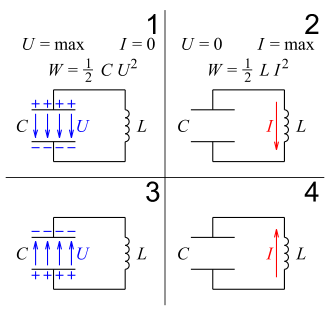
\includegraphics[width=0.382\textwidth]{pictures/schwing}
  \end{center}
\caption{Schwingungen}
\vspace{-50pt}
\end{wrapfigure}

Für
\marginnote{
\href{https://www.youtube.com/watch?v=KEgk-5s7VVM}{\qrcode{https://www.youtube.com/watch?v=KEgk-5s7VVM}}
}
die Auslenkung eines Massenpunktes $m$ gilt nach dem Hook'schen Gesetz
$$F=-kx$$
wobei $k$ die Federkonstante bezeichnet und $y$ die Auslenkung aus der Ruhelage. Die Bewegungsgleichung lautet daher
\begin{align*}
ma &= -ky\\
m\ddot{y} &= -ky
\end{align*}
was wir mit $\omega_0^2=\frac{k}{m}$ in der Form
$$\ddot{y}+\omega_0^2 y=0$$
schreiben. Als Lösungsansatz wählen wir
$$y(t)=Ce^{\omega t}.$$
Eingesetzt ergibt dies $\omega^2+\omega_0^2=0$ und damit
$$\omega_{1,2}=\pm \mathrm{i}\omega_0.$$
Wir erhalten also die beiden Lösungen
\begin{align*}
y_1(t) &= C_1\mathrm{e}^{\mathrm{i}\omega_0 t}\\
y_2(t) &= C_2\mathrm{e}^{-\mathrm{i}\omega_0 t},
\end{align*}
die für $\omega_0\neq0$ linear unabhängig sind. Die allgemeine Lösung der Differentialgleichung ist dann eine Linearkombination
$$y(t)=C_1\mathrm{e}^{\mathrm{i}\omega_0 t}+ C_2\mathrm{e}^{-\mathrm{i}\omega_0 t}.$$
Da $y(t)$ eine \emph{reelle} Funktion sein muss, impliziert das für komplexe Konstanten $C_1=C_2^*$. Wir setzen $C_1=a+\mathrm{i}b$ und $C_2=a-\mathrm{i}b$ und erhalten mit der Euler'schen Formel die allgemeine Lösung
$$y(t)=2a\cos(\omega_0 t)-2b\sin(\omega_0 t)$$
oder kürzer
$$y(t)=k_1\cos(\omega_0 t)+k_2\sin(\omega_0 t).$$
Unter Kenntnis des Additionstheorems
$$\sin(x+y)=\sin x\cos y+\sin y\cos x$$
lässt sich $k_1$ als $y_0\sin\varphi$ und $k_2$ als $y_0\cos\varphi$ auffassen, was
$$y(t)=y_0\sin(\omega_0 t+\varphi_0)$$
liefert.

\begin{figure}
\begin{center}

\scalebox{1.5}{
\begin{tikzpicture}[line cap=round,line join=round,>=triangle 45,x=0.8cm,y=1.0cm]
\draw [color=lightgray,dash pattern=on 1pt off 1pt, xstep=1.2566370614359172cm,ystep=1.0cm] (-0.96,-1.32) grid (7.74,1.24);
\draw[->,color=black] (-0.96,0) -- (7.74,0);
\foreach \x in {0.5,1,1.5,2}
\draw[shift={(\x*3.14,0)},color=black] (0pt,2pt) -- (0pt,-2pt) node[below] {\footnotesize $\x\pi$};
\draw[color=black] (7.5,0.03) node [anchor=south west] {$x$};
\draw[->,color=black] (0,-1.32) -- (0,1.24);
\foreach \y in {-1,1}
\draw[shift={(0,\y)},color=black] (2pt,0pt) -- (-2pt,0pt) node[left] {\footnotesize $\y$};
\draw[color=black] (0.07,1.11) node [anchor=west] {$y$};
\clip(-0.96,-1.32) rectangle (7.74,1.24);
\draw[smooth,samples=100,domain=-0.9570994940978063:7.741433389544653] plot(\x,{sin(((\x)+0.76)*180/pi)});
\end{tikzpicture}
}
\end{center}
\caption{Freie un\-ge\-dämpf\-te Schwingung}
\end{figure}

\subsection{Freie gedämpfte Schwingung}

Wie im vorangegangenen Kapitel betrachten wir eine Federschwingung; jetzt aber
\marginnote{
\href{https://www.youtube.com/watch?v=eXkSAAYvprc}{\qrcode{https://www.youtube.com/watch?v=eXkSAAYvprc}}
}
gedämpft durch eine Kraft, die wir proportional zur Geschwindigkeit des Massenpunktes annehmen. Dies beobachtet man zum Beispiel bei einer laminaren Strömung eines Mediums um den schwingenden Körper (Stoke'sche Reibung). Die Bewegungsgleichung lautet jetzt
$$ma=-ky-\alpha \dot{y}.$$
Umschreiben:
\begin{align*}
m\ddot{y}+\alpha \dot{y}+ky &= 0\\
\ddot{y} +\frac{\alpha}{m}\dot{y}+\frac{k}{m}y&=0\\
\ddot{y}+2\beta\dot{y}+\omega_0^2 y &=0
\end{align*}
mit $\frac{\alpha}{m}=2\beta$ und $\frac{k}{m}=\omega_0^2$.
Im Falle $\beta\geq0$ und $\omega_0^2\geq0$ wählen wir den Lösungsansatz
$$y(t)=Ce^{\omega t}.$$
Eingesetzt ergibt sich die charakteristische Gleichung
$$\omega^2+2\beta\omega+\omega_0^2=0$$
mit der Lösung
$$\omega_{1,2}=-\beta\pm\sqrt{\beta^2-\omega_0^2}.$$
Wegen der Präsenz von zwei Variablen, $\beta$ und $\omega_0$, müssen wir verschiedene Fälle unterscheiden.

\begin{description}
\item[Fall 1] Ist $\beta>\omega_0$, so haben wir starke Dämpfung; der sogenannte \definition{Kriechfall}. $\omega_1$ und $\omega_2$ sind somit reell und voneinander verschieden. Die Lösung in diesem Fall ist
$$y(t)=k_1\mathrm{e}^{\omega_1 t}+k_2\mathrm{e}^{\omega_2 t}.$$

Für $k_1=20, k_2=-20,\omega_1=-0.5$ und $\omega_2=-2.5$ ergibt sich folgendes Bild.

\begin{figure}
\begin{center}

\scalebox{1.2}{
\begin{tikzpicture}[line cap=round,line join=round,>=triangle 45,x=1.0cm,y=0.5cm]
\draw [color=lightgray,dash pattern=on 3pt off 3pt, xstep=1.57cm,ystep=1.0cm] (0,-1) grid (6.5,11);
\draw[->,color=black] (-0.5,0) -- (6.5,0);
\foreach \x in {0.5,1,1.5,2}
\draw[shift={(\x*3.14,0)},color=black] (0pt,2pt) -- (0pt,-2pt) node[below] {\footnotesize $\x\pi$};
\draw[color=black] (6.31,0.16) node [anchor=south west] { x};
\draw[->,color=black] (0,-2) -- (0,12);
\foreach \y in {2,4,6,8,10}
\draw[shift={(0,\y)},color=black] (2pt,0pt) -- (-2pt,0pt) node[left] {\footnotesize $\y$};
\draw[color=black] (0.05,11.21) node [anchor=west] { y};
\clip(-0.5,-2) rectangle (6.5,12);
\draw plot[raw gnuplot, id=func0] function{set samples 100; set xrange [0:6.4]; plot 20*2.71**(-0.5*x)-20*2.71**(-2.5*x)};
\end{tikzpicture}
}
\end{center}
\caption{Freie gedämpfte Schwingung: Kriech\-fall}
\end{figure}

\item[Fall 2] Mit $\beta=\omega_0$ erreicht man starke Dämpfung, der sogenannte \definition{aperiodische Grenzfall}; $\lambda_1=\lambda_2=-k<0$.
Als Lösung erhalten wir damit
$$y(t)=k_1\mathrm{e}^{-\beta t}+k_2t\mathrm{e}^{-\beta t}.$$
Der Bewegungsablauf gleicht also dem vom Fall 1. Unten ist der Verlauf für $k_1=0, k_2=10$ und $\beta=-2.5$ illustriert.

\begin{figure}
\begin{center}

\scalebox{1.5}{
\begin{tikzpicture}[line cap=round,line join=round,>=triangle 45,x=1.0cm,y=1.5cm]
\draw [color=lightgray,dash pattern=on 1pt off 1pt, xstep=1.57cm,ystep=0.75cm] (0,0) grid (6.5,1.7);
\draw[->,color=black] (-0.5,0) -- (6.5,0);
\foreach \x in {0.5,1,1.5,2}
\draw[shift={(\x*3.14,0)},color=black] (0pt,2pt) -- (0pt,-2pt) node[below] {\footnotesize $\x\pi$};
\draw[color=black] (6.23,0.03) node [anchor=south west] {$\omega t$};
\draw[->,color=black] (0,-0.5) -- (0,2);
\foreach \y in {0.5,1,1.5}
\draw[shift={(0,\y)},color=black] (2pt,0pt) -- (-2pt,0pt) node[left] {\footnotesize $\y$};
\draw[color=black] (0.05,1.86) node [anchor=west] {$x(t)$};
\clip(-0.5,-0.5) rectangle (6.5,2);
\draw plot[raw gnuplot, id=func0] function{set samples 100; set xrange [0:6.4]; plot 10*x*2.71**(-2.5*x)};
\end{tikzpicture}
}
\end{center}
\caption{Freie gedämpfte Schwingung: aperiodischer Grenzfall}
\end{figure}

\item[Fall 3] Schwache Dämpfung, einen sogenannten \definition{Schwingfall}, erhält man für $\beta<\omega_0$.
Dabei sind $\omega_1$ und $\omega_2$ konjugiert komplexe Wurzeln, $\omega_{1,2}=-\beta\pm\omega_1\mathrm{i}$ mit $\omega_1=\sqrt{\omega_0^2-\beta^2}$. Die Lösung ist
$$y(t)=\mathrm{e}^{-\beta t}(k_1\cos(\omega_1 t)+k_2\sin(\omega_1 t))$$
oder, ähnlich der Behandlung freier Schwingungen mittels Additionstheorem,
$$y(t)=A\mathrm{e}^{-\beta t}\sin(\omega_1 t+\varphi),$$
mit $A^2=k_1^2+k_2^2$ und $\tan\varphi=\frac{k_1}{k_2}$. Dies ist die gedämpfte harmonische Schwingung.

$\omega_1=\sqrt{\omega_0^2-\beta^2}$ zeigt, dass im Falle der gedämpften Schwingung die Kreisfrequenz $\omega_1$ kleiner als die Kreisfrequenz $\omega_0$ der freien Schwingung ist.

\begin{figure}
\begin{center}

\scalebox{1.5}{
\begin{tikzpicture}[line cap=round,line join=round,>=triangle 45,x=0.2cm,y=2.0cm]
\draw [color=lightgray,dash pattern=on 2pt off 2pt, xstep=0.3141592653589793cm,ystep=1.0cm] (-3,-1.2) grid (25.5,1.2);
\draw[->,color=black] (-3,0) -- (25.5,0);
\foreach \x in {-1.57,1.57,3.15,4.71,6.28,7.85,9.42,11,12.57,14.14,15.71,17.28,18.85,20.42,21.99,23.56,25.13}
\draw[shift={(\x,0)},color=black] (0pt,2pt) -- (0pt,-2pt);
\draw[color=black] (24.38,0.03) node [anchor=south west] { $\omega t$};
\draw[->,color=black] (0,-1.2) -- (0,1.2);
\foreach \y in {-1,-0.5,0.5,1}
\draw[shift={(0,\y)},color=black] (2pt,0pt) -- (-2pt,0pt) node[left] {\footnotesize $\y$};
\draw[color=black] (0.22,1.06) node [anchor=west] { $y(t)$};
\clip(-3,-1.2) rectangle (25.5,1.2);
\draw plot[raw gnuplot, id=func3] function{set samples 100; set xrange [0.1:25.1]; plot 2.71**(-0.1*x)*sin((3.14/180*x)*180/3.14)};
\draw[dash pattern=on 2pt off 2pt] plot[raw gnuplot, id=func4] function{set samples 100; set xrange [0.1:25.1]; plot 2.71**(-0.1*x)};
\draw[dash pattern=on 2pt off 2pt] plot[raw gnuplot, id=func5] function{set samples 100; set xrange [0.1:25.1]; plot -2.71**(-0.1*x)};
\end{tikzpicture}
}
\end{center}
\caption{Gedämpfte harmonische Schwingung}
\end{figure}
\end{description}


\subsection{Erzwungene Schwingung}
Wir
\marginnote{
\href{https://www.youtube.com/watch?v=3zc1PeyGRAY}{\qrcode{https://www.youtube.com/watch?v=3zc1PeyGRAY}}
}
betrachten eine gedämpfte Schwingung, die periodisch mit der Kraft $F=mB\cos(\omega_a t)$ angetrieben wird. Die Schwingungsgleichung lautet
$$\ddot{y}+2\beta\dot{y}+\omega_0^2y=B\cos(\omega_a t).$$
Dies ist eine inhomogene lineare Differentialgleichung zweiter Ordnung. Zur Lösung kommen wir wie gelernt

\begin{enumerate}[a)]
\item lösen der homogenen Gleichung
\item ergänzen der Lösung mit einer partikulären
\end{enumerate}

Die homogene Differentialgleichung wurde im Kapitel zur freien, gedämpften Schwingung hergeleitet. Für geringe Dämpfung ergab sich --- wenn wir nur den homogenen Teil benutzen ---
$$y_{hom}=Ae^{-\beta t}\sin(\omega_1 t+\varphi)$$
mit $\omega_1=\sqrt{\omega_0^2-\beta^2}$.

Um die allgemeine Lösung zu gewinnen, bleibt eine partikuläre Lösung der inhomogenen Differentialgleichung zu bestimmen. Als Ausgangspunkt dafür nutzen wir eine experimentelle Beobachtung: Das System schwingt demnach immer mit der Erregerfrequenz $\omega_a$, die Eigenfrequenz $\omega_1$ spielt mit der Zeit keine Rolle. Daher wählen wir den Lösungsansatz
$$y_{part}=C\sin(\omega_a t)+D\cos(\omega_a t).$$
Wir kommen mit einer einfachen Rechnung zum Ziel, wenn wir einen komplexen Ansatz wählen. Wegen $A\cos(\omega_a t)=\mathrm{Re}(A\mathrm{e}^{\mathrm{i}\omega_a t})$ wählen wir
$$y_{part}=C\mathrm{e}^{\mathrm{i}\omega_a t}.$$
Damit ergibt sich der komplexe Ansatz
$$-\omega_a^2C\mathrm{e}^{\mathrm{i}\omega_a t}+2\beta\mathrm{i}\omega_a C\mathrm{e}^{\mathrm{i}\omega_a t}+\omega_0^2C\mathrm{e}^{\mathrm{i}\omega_a t}=A\mathrm{e}^{\mathrm{i}\omega_a t}.$$
Das heisst $C(\omega_0^2-\omega_a^2+2\mathrm{i}\beta\omega_a)=A$. Zur Analyse unterscheidet man zwei Fälle --- Klammerausdruck gleich oder ungleich $0$.

\begin{description}
\item[Fall 1] Sei $\omega_0^2-\omega_a^2+2\mathrm{i}\beta\omega_a\neq0$, das heisst $\mathrm{Re}(\omega_0^2-\omega_a^2)\neq0$ oder $\mathrm{Im}(2\mathrm{i}\beta\omega_a)\neq0$. Somit
$$C=\frac{A}{\omega_0^2-\omega_A^2+\mathrm{i}\cdot 2\beta\omega_a},$$
was komplex erweitert
$$
C=\frac{A(\omega_0^2-\omega_a^2)}{(\omega_0^2-\omega_a^2)^2+4\beta^2\omega_a^2}-\mathrm{i}\frac{2\beta\omega_a A}{(\omega_0^2-\omega_a^2)^2+4\beta^2\omega_a^2}
$$
ergibt. Damit erhalten wir für unseren Ansatz
$$
\mathrm{Re}(C\mathrm{e}^{\mathrm{i}\omega_a t})=\frac{A(\omega_0^2-\omega_a^2)}{(\omega_0^2-\omega_a^2)^2+4\beta^2\omega_a^2}\cos(\omega_a t)+\frac{2\beta\omega_a A}{(\omega_0^2-\omega_a^2)^2+4\beta^2\omega_a^2}\sin(\omega_a t).
$$
Eine weitere Vereinfachung mittels des Additionstheorems
$$\cos(x+y)=\cos(x)\cos(y)-\sin(x)\sin(y)$$
kann vorgenommen werden, wenn man den Faktor
$$\frac{A}{\sqrt{(\omega_0^2-\omega_a^2)^2+4\beta^2\omega_a^2}}$$
ausklammert. Erst dann lässt sich die für die Winkelfunktion notwendige Bedingung $\sin^2(x)+\cos^2(x)=1$ erfüllen. Es folgt
$$
\mathrm{Re}(C\mathrm{e}^{\mathrm{i}\omega_a t})=\frac{A}{\sqrt{(\omega_0^2-\omega_a^2)^2+4\beta^2\omega_a^2}}\cdot(\cos(\alpha)\cos(\omega_a t)-\sin(\alpha)\sin(\omega_a t))
$$
mit
$$\cos(\alpha)=\frac{(\omega_0^2-\omega_a^2)}{\sqrt{(\omega_0^2-\omega_a^2)^2+4\beta^2\omega_a^2}}$$
und
$$\sin(\alpha)=-\frac{2\beta\omega_a}{\sqrt{(\omega_0^2-\omega_a^2)^2+4\beta^2\omega_a^2}}.$$
Wir haben endlich
\begin{align*}
y_{part}&=\mathrm{Re}(C\mathrm{e}^{\mathrm{i}\omega_a t})\\
&=\frac{A}{\sqrt{(\omega_0^2-\omega_a^2)^2+4\beta^2\omega_a^2}}\cos(\omega_a t+\varphi_a)
\end{align*}
mit $\tan(\alpha)=-\frac{2\beta\omega_a}{\omega_0^2-\omega_a^2}$ und damit für die Lösungsgesamtheit die allgemeine Lösung
$$
y(t)=A\mathrm{e}^{-\beta t}\sin(\omega_1 t+\varphi)+\frac{A}{\sqrt{(\omega_0^2-\omega_a^2)^2+4\beta^2\omega_a^2}}\cos(\omega_a t+\varphi_a)
$$

\item[Fall 2] Man erhält für $\omega_0^2=\omega_a^2$ mit $\beta=0$ Resonanz. Wegen des Anwachsens der Amplitude versucht man einen partikulären Ansatz mit Wachstum,
$$y_{part}=Ct\mathrm{e}^{\mathrm{i}\omega_0 t}.$$
Nach Einsetzen folgt
$$2C\mathrm{i}\omega_0=A$$
oder
$$C=-\frac{A}{2\omega_0}\mathrm{i}.$$
Wir erhalten
$$y_{part}=\mathrm{Re}(Ct\mathrm{e}^{\mathrm{i}\omega_0 t})=\frac{A}{2\omega_0}t\sin(\omega_0 t)$$
und für die Lösungsgesamtheit
$$
y(t)=\frac{A}{2\omega_0}t\sin(\omega_0 t)+k_1\cos(\omega_0 t)+k_2\sin(\omega_0 t).
$$

\end{description}

\clearpage

\appendix

\section{Bevölkerungswachstum}

Ein
\marginnote{
\href{https://www.youtube.com/watch?v=knQOOsgjbYg}{\qrcode{https://www.youtube.com/watch?v=knQOOsgjbYg}}
}
einfaches Modell zur Beschreibung einer Population $p$ ohne natürliche Feinde ist, dass sowohl die Geburtenzahl, wie auch die Sterbezahl proportional zur Grösse der Bevölkerung sind. Dann gibt es eine Geburtenrate $B$, eine Sterberate $D$ und $p$ genügt der Gleichung
\begin{equation}\label{eq:population}
\dot{p}=Bp-Dp.
\end{equation}
Mit $\beta =B-D$ in \eqref{eq:population} erhält man einen Wachstumsprozess vom Typ \eqref{eq:radiozerfall} mit Verdoppelungszeit $T=\ln(2)/\beta $.

Ein schwerer Nachteil dieses Modells ist die Vorhersage grenzenlosen Wachstums. Dies kann wegen der Endlichkeit aller Dinge nicht vorliegen. Nun erweitert man das Modell durch einen sogenannten Stressfaktor $S$, der proportional zur Anzahl Begegnungen von Individuen der Bevölkerung ist. Damit hat man
\begin{equation}\label{eq:populationstress}
\dot{p}=\beta  p-Sp^2.
\end{equation}
Mit $p(t)=\frac{\beta}{S}$
verfügt man über eine konstante Lösung. Man bekommt die Lösung für einen beliebigen Anfangswert mit der Methode der Trennung der Veränderlichen.

Nehmen wir an, es gibt eine Lösung $p(t)$ mit $p_0\neq\beta /S$. Ist $\beta  p-Sp^2\neq0$ liefert \eqref{eq:populationstress}
$$\frac{\mathrm{d}p}{\mathrm{d}t}\frac{1}{\beta  p-Sp^2}=1.$$
Integration von $t_0$ bis $t$ ergibt
$$\int_{t_0}^t\frac{\mathrm{d}p(s)}{\mathrm{d}t}\frac{\mathrm{d}s}{\beta  p(s)-Sp(s)^2}=\int_{t_0}^t\,\mathrm{d}s=t-t_0.$$
Ist $\beta  p-Sp^2\neq0$, so ist auch $p'\neq0$ und die linke Seite ergibt mit der Substitutionsregel
$$\int_{p_0}^p\frac{\mathrm{d}z}{\beta  z-Sz^2}.$$
Dieser Ausdruck wird mittels einer Partialbruchzerlegung integriert.

\begin{uebenv}{partbruch}
Zeige, dass mit $K=\beta/S$
$$\frac{1}{\beta  z-Sz^2}=\frac{1}{\beta }\cdot\left(\frac{1}{z}+\frac{1}{K-z}\right)$$
gilt.
\end{uebenv}

Wir erhalten mit $K=\beta/S$ für das Integral
\begin{align*}
\frac{1}{\beta }\int_{p_0}^p\frac{1}{z}+\frac{1}{K-z}\,\mathrm{d}z &=\frac{1}{\beta }\left(\ln\left(\frac{|p|}{|p-K|}\right)-\ln\left(\frac{|p_0|}{|p_0-K|}\right)\right).
\end{align*}

\begin{uebenv}{partintfurther}
Zeige: Wegen $p_0,p>0$ erhält man für den vorangehenden Ausdruck die Form
$$\frac{p(p_0-K)}{(p-K)p_0}=\mathrm{e}^{\beta (t-t_0)}.$$
\end{uebenv}

Daraus folgt
\begin{equation}\label{eq:bruch}
p(1-B)=-BK.
\end{equation}
Schliesslich erhalten wir die Lösung
$$p(t)=\frac{Kp_0}{p_0-\mathrm{e}^{-\beta (t-t_0)}(p_0-K)}.$$

\begin{uebenv}{logwachstumexplizit}
Leite die Lösung her, indem du \eqref{eq:bruch} nach $p$ auflöst, den Bruch ausschreibst und danach mit $\mathrm{e}^{-\beta (t-t_0)}$ erweiterst.
\end{uebenv}

\begin{uebenv}{explizitelsganalysis}
Untersuche die Qualität der Lösung. Erfüllt $p(t_0)$ die Erwartungen. Wie sieht's in ferner Zukunft aus, d.h. $t\to\infty$?
\end{uebenv}

\clearpage

\subsection{Notizen zu den Übungen}

\begin{lsg}{partbruch}
    Zuerst
    $$\frac{1}{\beta z-Sz^2}=\frac{1}{\beta z-\frac{\beta}{K}z^2}=\frac{1}{\beta(z-\frac{1}{K}z^2)}=\frac{1}{\beta}\cdot\frac{1}{z(1-\frac{1}{K}z)}.$$
    Und nun folgt die Partialbruchzerlegung. Ansatz
    \begin{align*}
        \frac{K}{z(K-z)} &= \frac{a_1}{z}+\frac{a_2}{K-z}\\
        K &= a_1(K-z)+a_2z\\
        &= a_1K+z(a_2-a_1)
    \end{align*}
    und ein Vergleich zeigt $a_1=1$ und auch $a_2=1$. Also gilt $\frac{1}{\beta  z-Sz^2}=\frac{1}{\beta }\cdot\left(\frac{1}{z}+\frac{1}{K-z}\right)$.
\end{lsg}
\begin{lsg}{partintfurther}
    Mit der Logarithmenregel für Subtraktion folgt
    $$\frac{1}{\beta}\left(\ln\left(\frac{|p||p_0-K|}{|p-K||p_0|}\right)\right)=t-t_0\Leftrightarrow \ln\left(\frac{|p||p_0-K|}{|p-K||p_0|}\right)=\beta(t-t_0).$$
    Da wir $p(s)\neq K$ sowie $p\neq0\neq p_0$ $\forall s\in[t_0,t]$ fordern, folgt dass $p-K$ und $p_0-K$ das gleiche Vorzeichen haben, denn aus $p(s)<K\;\forall s\in[t_0,t]$ folgt $p_0<K$ und vice versa. Also gilt die Behauptung nach Exponentiation beider Seiten zur Basis $\mathrm{e}$.
\end{lsg}
\begin{lsg}{logwachstumexplizit}
    Es ist
    $$p(p_0-K)=pp_0\mathrm{e}^{\beta(t-t_0)}-Kp_0\mathrm{e}^{\beta(t-t_0)}$$
    und daraus folgt
    \begin{align*}
        p(p_0-K)\mathrm{e}^{-\beta(t-t_0)}-pp_0 &= Kp_0\\
        p(t) &= \frac{Kp_0}{p_0+(K-p_0)\mathrm{e}^{-\beta(t-t_0)}}
    \end{align*}
\end{lsg}
\begin{lsg}{explizitelsganalysis}
    $p(t_0)=\frac{Kp_0}{p_0+(K-p_0)\mathrm{e}^{-\beta(t_0-t_0)}}=\frac{Kp_0}{p_0+(K-p_0)}=p_0$ wie erwartet. Im Langzeitverhalten geht $\mathrm{e}^{-\beta(t-t_0)}\to0$, also $\lim_{t\to\infty}\frac{Kp_0}{p_0+(K-p_0)\mathrm{e}^{-\beta(t-t_0)}}=\frac{Kp_0}{p_0}=K$.
\end{lsg}

\clearpage

\section{Lineare Differentialgleichungssysteme}

\begin{bsp}
Gegeben sei das lineare Differentialgleichungssystem
\marginnote{
\href{https://www.youtube.com/watch?v=Tbhw2Se259U}{\qrcode{https://www.youtube.com/watch?v=Tbhw2Se259U}}
}
erster Ordnung
\begin{align*}
y_1'&=7y_1-5y_2\\
y_2'&=4y_1-2y_2
\end{align*}
das heisst
$$\vec{y}\,'=
\begin{pmatrix}
7 & -5\\
4 & -2
\end{pmatrix}
\vec{y}.$$
Im Unterricht wurde gezeigt, dass die Lösung dieses Systems darauf hinaus läuft, dass man die Eigenwerte und Eigenvektoren der zugehörigen Koeffizientenmatrix kennt.

Wir finden die Eigenwerte via
$$(\lambda-7)(\lambda+2)+20=0$$
oder mit dem charakteristischen Polynom $\chi_A(\lambda)$.
Das ergibt $\lambda_1=2$ und $\lambda_2=3$. Daraus erhält man die Eigenvektoren
$$\vec{v_1}=\begin{pmatrix}
    1\\1
\end{pmatrix}\quad\text{und}\quad\vec{v_2}=\begin{pmatrix}
    5\\4
\end{pmatrix}.$$

Dies liefert das Fundamentalsystem der Lösungen
$$\begin{pmatrix}
    y_1\\y_2
\end{pmatrix}=c_1\mathrm{e}^{2x}\begin{pmatrix}
    1\\1
\end{pmatrix}+c_2\mathrm{e}^{3x}\begin{pmatrix}
    5\\4
\end{pmatrix}.$$
\end{bsp}

\begin{uebenv}{quickewundev}
Rechne Eigenwerte und Eigenvektoren nach.
\end{uebenv}

\begin{uebenv}{dglsyscheck}
Zeige, dass $\begin{pmatrix}
    y_1\\y_2
\end{pmatrix}$ das Gleichungssystem erfüllt.
\end{uebenv}

\clearpage

\subsection{Notizen zu den Übungen}

\begin{lsg}{quickewundev}
    Das charakteristische Polynom $\chi_A(\lambda)=\lambda^2-\mathrm{Tr}(A)\lambda+\det(A)=\lambda^2-5\lambda+6=(\lambda -2)(\lambda-3)$ muss gleich $0$ gesetzt werden. Also lösen $\lambda_1=2$ und $\lambda_2=3$ die Forderung.

    Für die Eigenvektoren erhält man aus der zweiten Zeile mit $\lambda_1=2$ folglich $4x-4y=0$, also $y=x$ bzw. $\begin{pmatrix}
        1\\1
    \end{pmatrix}$ und für $\lambda_2=3$ die Gerade $4x-5y=0$, also $y=\frac{4}{5}x$ bzw. $\begin{pmatrix}
        5\\4
    \end{pmatrix}$.
\end{lsg}
\begin{lsg}{dglsyscheck}
    Es sind $y_1=c_1\mathrm{e}^{2x}+5c_2\mathrm{e}^{3x}$ bzw. $y_2=c_1\mathrm{e}^{2x}+4c_2\mathrm{e}^{3x}$ und die zugehörigen Ableitungen $y_1'=2c_1\mathrm{e}^{2x}+15\mathrm{e}^{3x}$ bzw. $y_2'=2c_2\mathrm{e}^{2x}+12\mathrm{e}^{3x}$. Auf beiden Seiten eingesetzt und \checkmark.
\end{lsg}

\clearpage

\section{Die Traktrix}

\begin{wrapfigure}{r}{0.4\textwidth}
\vspace{-5pt}
\begin{center}
\definecolor{xdxdff}{rgb}{0.3,0.3,0.3}
\scalebox{0.9}{
\begin{tikzpicture}[line cap=round,line join=round,>=triangle 45,x=1.0cm,y=1.0cm]
\draw[->,color=black] (-1.9,0) -- (4.94,0);
\foreach \x in {-1,1,2,3,4}
\draw[shift={(\x,0)},color=black] (0pt,-2pt);
\draw[color=black] (4.6,0.08) node [anchor=south west] { x};
\draw[->,color=black] (0,-1.94) -- (0,6.3);
\foreach \y in {-1,1,2,3,4,5,6}
\draw[shift={(0,\y)},color=black] (2pt,0pt) -- (-2pt,0pt);
\draw[color=black] (-0.1,5.9) node [anchor=east] { y};
\clip(-1.9,-1.94) rectangle (4.94,6.3);
\draw[smooth,samples=100,domain=0.02:2.9] plot(\x,{3*ln((3+(9-(\x)^2)^0.5)/(\x))-(9-(\x)^2)^0.5});
\draw (0,4)-- (1.5,1.35);
\draw [dotted] (0,1.35)-- (1.5,1.35);
\draw [dotted] (1.5,1.35)-- (1.5,0);
\begin{scriptsize}
\fill [color=xdxdff] (0,4) circle (1.5pt);
\draw[color=xdxdff] (0.14,4.26) node {$Z$};
\fill [color=xdxdff] (1.5,1.35) circle (1.5pt);
\draw[color=xdxdff] (1.64,1.62) node {$P$};
\end{scriptsize}
\end{tikzpicture}
}
\end{center}
\caption{Die Traktrix}
\vspace{-5pt}
\end{wrapfigure}
In
\marginnote{
\href{https://www.youtube.com/watch?v=7c4ajQ6n39w}{\qrcode{https://www.youtube.com/watch?v=7c4ajQ6n39w}}
}
der $xy$-Ebene ziehe man einen Punkt $P(x|y)$ an einer Schnur $PZ$ der Länge $a$. $Z$ soll auf der positiven $y$-Achse fortrücken, und zu Beginn befinde sich $P$ in $(a,0)$. Welche Kurve beschreibt $P$?
Wir suchen eine Funktion $y=y(x)$ mit $|Z-P|=a$. Betrachtet man den Steigungswinkel erhält man für den Punkt $P$
$$y'=-\frac{Z-y}{x}.$$
Ferner gilt
$$Z-y=\sqrt{a^2-x^2}$$ und damit
$$y'=-\frac{\sqrt{a^2-x^2}}{x}.$$
Mit der Bedingung $y(a)=0$ erhält man als Lösung
$$y(x)=a\cdot\ln\left(\frac{a+\sqrt{a^2-x^2}}{x}\right)-\sqrt{a^2-x^2}.$$

\begin{uebenv}{lsgtraktrix}
Überprüfe die Lösung.
\end{uebenv}

\begin{lsg}{lsgtraktrix}
    Wir nehmen die Lösung $y(x)=a\ln\left(\frac{a+\sqrt{a^2-x^2}}{x}\right)-\sqrt{a^2-x^2}$ und leiten ab:
    \begin{align*}
        y' &= a\frac{x}{a+\sqrt{a^2-x^2}}\cdot\frac{\frac{1}{2\sqrt{a^2-x^2}}\cdot x(-2x)-(a+\sqrt{a^2-x^2})\cdot1}{x^2}-\frac{1}{2\sqrt{a^2-x^2}}\cdot(-2x)\\
        &= \frac{ax}{a+\sqrt{a^2-x^2}}\cdot\frac{\frac{-x^2}{\sqrt{a^2-x^2}}-(a+\sqrt{a^2-x^2})}{x^2}+\frac{x}{\sqrt{a^2-x^2}}\\
        &= \frac{ax}{a+\sqrt{a^2-x^2}}\cdot\left( -\frac{1}{\sqrt{a^2-x^2}}-\frac{a+\sqrt{a^2-x^2}}{x^2}\right)+\frac{x}{\sqrt{a^2-x^2}}\\
        &= -\frac{ax}{(a+\sqrt{a^2-x^2})\sqrt{a^2-x^2}}-\frac{a}{x}+\frac{x}{\sqrt{a^2-x^2}}\\
        &= \frac{-a^2\sqrt{a^2-x^2}-a(a^2-x^2)+x^2\sqrt{a^2-x^2}}{x(a+\sqrt{a^2-x^2})\sqrt{a^2-x^2}}\\
        &= -\frac{a^2+a\sqrt{a^2-x^2}-x^2}{x(a+\sqrt{a^2-x^2})}\\
        &= -\frac{a(a+\sqrt{a^2-x^2})-(a+\sqrt{a^2-x^2})(a-\sqrt{a^2-x^2})}{x(a+\sqrt{a^2-x^2})}\\
        &= -\frac{\sqrt{a^2-x^2}}{x}
    \end{align*}
\end{lsg}

\clearpage

\section{Isoklinenverfahren}

Über die Differentialgleichung
$$y'=f(x,y)$$
ist jedem Punkt der $xy$-Ebene eine Richtung $y'=\tan(\alpha)$ zugeordnet. Wählt man für $y'$ einen festen Wert,
$$y'=c=f(x,y),$$
so beschreibt diese Gleichung eine Kurve in der Ebene.
Diese Kurven heissen \definition{Isoklinen}, also Kurven gleicher Neigung. Durch Zeichnung von genügend vielen Richtungsstrecken erhält man ein Richtungsfeld, in das man näherungsweise Lösungskurven der Differentialgleichung eintragen kann.

\begin{uebenv}{isoklinen}
Zeichne für
$$y'=-\frac{y}{x}$$
einige Isoklinen und damit mögliche Lösungskurven.
\end{uebenv}

\begin{lsg}{isoklinen}
    Man zeichnet an einigen Stellen Steigungen vom Wert $-\frac{y}{x}$ und ist fertig.

\begin{center}
    \begin{tikzpicture}
    % Achsen
    \draw[->] (-3,0) -- (3,0) node[above right] {$x$};
    \draw[->] (0,-3) -- (0,3) node[above left] {$y$};
    
    % Isoklinenfeld
    \foreach \x in {-2,-1.5,...,2} {
        \foreach \y in {-2,-1.5,...,2} {
            \ifthenelse{\lengthtest{\x pt = 0 pt}}{}{ % Ausschluss von x=0
                \pgfmathsetmacro{\m}{-\y/\x} % Steigung m = -y/x
                \pgfmathsetmacro{\dx}{0.2} % Schrittweite x
                \pgfmathsetmacro{\dy}{\m*\dx} % Schrittweite y
                \draw[thick] (\x-\dx, \y-\dy) -- (\x+\dx, \y+\dy);
            }
        }
    }
\end{tikzpicture}
\end{center}
\end{lsg}

\clearpage

\section{Die schwingende Saite}

Bei einer schwingenden Saite sucht man eine Funktion $u$, die die Auslenkung zum Zeitpunkt $t$ an der Stelle $x$ beschreibt, $u(t,x)$.
Ohne Begründung gebe ich die zugrundeliegende partielle Differentialgleichung an:
\begin{equation}\label{eq:saite}
\frac{\partial^2u}{\partial t^2}=\lambda^2\frac{\partial^2u}{\partial x^2}.
\end{equation}
Die Saite sei an den Endpunkten $x=0$ bzw. $x=\pi$ fixiert. Damit erhält man die Randbedingungen $u(t,0)=u(t,\pi)=0$. Der Einfachheit halber setzen wir $\lambda=1$.
Mit dem Ansatz $u(t,x)=v(x)\cdot w(t)$
erhalten wir die Beziehung $v(x)\ddot{w}(t)=v''(x)w(t)$.
Betrachten wir einen Punkt $(t,x)$, in dem beide Funktionen nicht verschwinden, so können wir
$$\frac{w''(t)}{w(t)}=\frac{v''(x)}{v(x)}$$
schreiben. Da die beiden Seiten von verschiedenen Variablen abhängen und für alle $x,t$ im Definitionsbereich erfüllt sein sollen, müssen sie konstant und gleich sein. Also in der Art
\begin{align*}
\ddot{w}&=-Kw\\
v''&=-Kv
\end{align*}
mit $K>0$. Das Vorzeichen ist wiederum physikalisch motiviert. Sonst erhält man keine zeitlich periodische Lösung. Wie in \eqref{eq:mathpendel} lautet eine Lösung der zweiten Gleichung
$$v(x)=c_1\cos(\sqrt{K}x)+c_2\sin(\sqrt{K}x).$$

\begin{uebenv}{saitenb}
Überlege dir, dass mit den Randbedingungen der Cosinusterm verschwindet und $K=n^2$ mit $n\in\mathbb{N}$ gelten muss, so dass also $v(x)=c_2\sin(nx)$ wird.
\end{uebenv}

Damit kann man eine Schar von Lösungen der Gleichung \eqref{eq:saite} angeben, nämlich
$$u(t,x)=\sum_{n=0}^\infty\left(d_n^1\cos(nt)+d_n^2\sin(nt)\right)\sin(nx).$$

\begin{uebenv}{saitefulllsg}
Geht man von einer Ausgangsauslenkung aus der Ruhelage mit Anfangsgeschwindigkeit $0$ aus, so erhält man
$$u(t,x)=\sum_{n=0}^\infty d_n\cos(nt)\sin(nx).$$
\end{uebenv}

\begin{figure}[h]
    \centering
    \begin{tikzpicture}
\begin{axis}[
  	%hide axis,
  	title={Schwingende Saite als 1. Oberschwingung},
  	grid=both,
	xlabel=$x$,ylabel=$t$,
	mesh/interior colormap name=hot,
	colormap/blackwhite, 
 ]
  \addplot3[domain=-pi:pi,surf,samples=50]
  	{sin(deg(x))*cos(deg(2*y))};
\end{axis}
\end{tikzpicture}
    \caption{Potential $u(x,t)=\sin(x)\cdot\cos(2t)$ der schwingenden Saite fixiert bei $-\pi$ und $\pi$}
    \label{fig:saite}
\end{figure}

\begin{lsg}{saitenb}
    Aus $v(0)=0$ folgt $c_1=0$ und $v(\pi)=c_2\sin(\sqrt{K}\pi)=0$ heisst $\sqrt{K}=n\in\mathbb{N}_0$, also $K=n^2$. Daraus folgt unmittelbar die Behauptung.
\end{lsg}
\begin{lsg}{saitefulllsg}
    Die Geschwindigkeit ist
    $$v_x(t)=\frac{\partial u(t,x)}{\partial t}=\sum_{n=0}^\infty (-d_n^1n\sin(nt)+d_n^2n\cos(nt))\sin(nx).$$
    Wegen
    $$v_x(0)=\frac{\partial u(0,x)}{\partial t}\stackrel{!}{=}0$$
    muss dann $d_n^2=0$ sein und dies führt direkt zur Behauptung.
\end{lsg}

\clearpage

\section{Die Wärmeleitungsgleichung}

Wir betrachten die eindimensionale Wärme\-lei\-tungs\-gleichung, die die Temperaturentwicklung eines Stab der Länge $l$ modelliert. Für $x\in(0,l)$ und $t\in\mathbb{R}$ sei $u(x,t)$ die Temperatur des Stabes zum Zeitpunkt $t$ an der Stelle $x$. Die Anfangsverteilung der Temperatur sei durch eine Funktion $u(x,0)$ gegeben. Zum einen kann man annehmen, dass man an den Enden eine feste Temperatur $T$ hat, o.E.d.A. nehmen wir $T=0$
an, eine vollständige Isolierung keine Temperaturänderung über die Zeit: $u_x(0,t)=u_x(l,t)=0$ für alle $t\in\mathbb{R}$. An der
Stelle $(x,t)$ ist dabei die Differentialgleichung
$$\frac{\partial u}{\partial t}=k\frac{\partial^2 u}{\partial^2 x}$$
erfüllt. Wiederum setzen wir $k=1$ und brauchen den Separationsansatz $u(x,t)=v(x)w(t)$. Man erhält
$$\frac{\dot{w}}{w}=\frac{v''}{v}=\lambda.$$
Hier lautet eine mögliche Lösung $u(x,t)=\mathrm{e}^{\lambda t}(c_1\cos(\sqrt{\lambda}x)+c_2\sin(\sqrt{\lambda}x))$, die man wie oben ausrechnet. Aus der Randbedingung links ergibt sich $c_1=0$, und die Bedingung rechts liefert $\sin(\sqrt{\lambda}l)=0$, also
$$\lambda=\frac{n^2\pi^2}{l^2}$$
für ein $n\in\mathbb{N}$. Da man beliebige Summen bzw. Reihen bilden kann, lautet eine allgemeinere Lösung
$$u(x,t)=\sum_{n=0}^\infty c_n\mathrm{e}^{\frac{n^2\pi^2}{l^2}t}\sin\left(\frac{n\pi}{l}x\right).$$
\marginnote{
\href{https://www.youtube.com/watch?v=QY7fD_fFYnk}{\qrcode{https://www.youtube.com/watch?v=QY7fD_fFYnk}}
}

\clearpage

\section{Das elektrische Feld}

Sei $\vec{E}$ ein elektrisches Feld in der Ebene.
\marginnote{
\href{https://youtu.be/0zcRz1kphBQ}{\qrcode{https://youtu.be/0zcRz1kphBQ}}
}
Sei $U$ das Potential dieses Feldes. Also $\vec{E}=-\nabla U$, wobei $U$ eine Funktion der beiden unabhängigen Veränderlichen $x,y$ sei. Welches sind die Linien, längs denen das Potential konstant ist, die \definition{Äquipotentiallinien}?
Um die Äquipotentiallinien zu finden, geben wir uns eine, zunächst beliebige, Konstante $c$ vor und stellen die Frage, wo ist $U=c$? Die Annahme, dass diese Linie durch $y = y(x)$ zu beschreiben ist, führt auf
$$\frac{\partial U}{\partial x}+\frac{\partial U}{\partial y}\frac{\mathrm{d}y}{\mathrm{d}x}=0.$$
Dies ist ein Beispiel einer sogenannten exakten Differentialgleichung.

\begin{uebenv}{efeldexakt}
Überlege kurz, dass obige Bedingung sinnvoll ist.
\end{uebenv}

\begin{cdef}[exakte Differentialgleichung]
Die
\marginnote{
\href{https://www.youtube.com/watch?v=haiyzr8B7_A}{\qrcode{https://www.youtube.com/watch?v=haiyzr8B7_A}}
}
Differentialgleichung der Form
\begin{equation}\label{eq:exakt}
P(x,y)\frac{\mathrm{d}y}{\mathrm{d}x}+Q(x,y)=0
\end{equation}
heisst exakt, wenn es eine Funktion $F:\mathbb{R}^2\supset\mathbb{G}\longrightarrow\mathbb{R}$, ein sogenanntes Potential, gibt, so dass
\begin{equation}\label{eq:exaktbed}
P(x,y)=\frac{\partial U}{\partial y}\quad\text{und}\quad Q(x,y)=\frac{\partial U}{\partial x}.
\end{equation}
\end{cdef}

Aus $F_{xy}=F_{yx}$ erhält man unmittelbar die notwendige Bedingung $P_x=Q_y$ für die Exaktheit der Gleichung. Diese Bedingung nennt man \definition{Integrabilitätsbedingung}. Ist bei einer Gleichung der Form \eqref{eq:exakt} die Bedingung \eqref{eq:exaktbed} nicht erfüllt, so ist es manchmal möglich, einen \definition{integrierenden Faktor} zu finden. Dies ist eine Funktion $M(x,y)$, so dass $MP$ bzw. $MQ$ die Bedingung \eqref{eq:exaktbed} erfüllen.

\begin{lsg}{efeldexakt}
    Da wir Äquipotentiallinien suchen, müssen die Richtungsableitungen $0$ ergeben.
\end{lsg}

\clearpage

\section{Bogenlänge}

Zur Herleitung der Formel betrachten wir den Graphen einer im Intervall $[a,b]$ differenzierbaren Funktion $f$. Sei $L_a(x)$ die Länge des Bogens von der Stelle $a$ bis zur Stelle $x$; betrachte auch Abbildung \ref{abb:bogenlaenge} auf Seite \pageref{abb:bogenlaenge}.

\begin{figure}
\begin{center}
\scalebox{1.3}{
\begin{tikzpicture}[line cap=round,line join=round,>=triangle 45,x=0.95cm,y=1.0cm]
\draw[->,color=black] (-0.52,0) -- (6.82,0);
\foreach \x in {,1,2,3,4,5,6}
\draw[shift={(\x,0)},color=black] (0pt,2pt) -- (0pt,-2pt);
\draw[color=black] (6.48,0.08) node [anchor=south west] {$x$};
\draw[->,color=black] (0,-0.92) -- (0,4.56);
\foreach \y in {,1,2,3,4}
\draw[shift={(0,\y)},color=black] (2pt,0pt) -- (-2pt,0pt);
\draw[color=black] (0.1,4.16) node [anchor=west] {$y$};
\clip(-0.52,-0.92) rectangle (6.82,4.56);
\draw[smooth,samples=100,domain=1.1:6.8] plot(\x,{ln((\x)-1)+2});
\draw [dotted] (1.57,1.44)-- (1.57,0);
\draw [dotted] (2.74,0)-- (2.74,2.55);
\draw [dotted] (4.71,3.31)-- (4.71,0);
\draw (2.74,2.55)-- (4.71,2.55);
\draw (2.74,2.55)-- (4.71,3.31);
\draw (4.71,3.31)-- (4.71,2.55);
\draw (3.54,2.5) node[anchor=north west] {$ \Delta x $};
\draw (4.7,3.2) node[anchor=north west] {$ \Delta y $};
\begin{scriptsize}
\fill [color=darkblue] (1.57,0) circle (1.5pt);
\draw[color=darkblue] (1.58,-0.24) node {$a$};
\fill [color=darkblue] (2.74,0) circle (1.5pt);
\draw[color=darkblue] (2.72,-0.24) node {$x$};
\fill [color=darkblue] (4.71,0) circle (1.5pt);
\draw[color=darkblue] (4.7,-0.24) node {$x+\Delta x$};
\fill [color=darkblue] (5.7,0) circle (1.5pt);
\draw[color=darkblue] (5.7,-0.24) node {$b$};
\fill [color=gray] (1.57,1.44) circle (1.5pt);
\draw[color=gray] (1.38,1.72) node {$A$};
\fill [color=gray] (2.74,2.55) circle (1.5pt);
\draw[color=gray] (2.5,2.7) node {$P$};
\fill [color=gray] (4.71,3.31) circle (1.5pt);
\draw[color=gray] (4.64,3.6) node {$Q$};
\end{scriptsize}
\end{tikzpicture}
}
\end{center}
\caption{Illustration der Bogenlänge einer Funktion $f$}\label{abb:bogenlaenge}
\end{figure}

Dann ist $\hat{AQ}=L_a(x+\Delta x)$ und $\hat{PQ}=\hat{AQ}-\hat{AP}=L_a(x+\Delta x)-L_a(x)$. Aus der Graphik erkennt man $\overline{PQ}\leq\hat{PQ}$. Mit Hilfe des Satzes von Pythagoras folgt
$$
\overline{PQ} =\sqrt{\Delta x^2+\Delta y^2}=\sqrt{\Delta x^2\left(1+\frac{\Delta y^2}{\Delta x^2}\right)}=\Delta x\sqrt{1+\frac{\Delta y^2}{\Delta x^2}}
$$
Daraus folgt
$$\Delta x\sqrt{1+\frac{\Delta y^2}{\Delta x^2}}\leq L_a(x+\Delta x)-L_a(x)$$
und nach Division mit $\Delta x$
$$\sqrt{1+\frac{\Delta y^2}{\Delta x^2}}\leq\frac{L_a(x+\Delta x)-L_a(x)}{\Delta x}.$$
Nun lassen wir $Q$ gegen $P$ gehen:
$$\lim_{\Delta x\to0}\frac{\Delta y^2}{\Delta x^2}=f'(x)^2$$
und
$$\lim_{\Delta x\to0}\frac{L_a(x+\Delta x)-L_a(x)}{\Delta x}=L_a'(x)$$
wobei nun Gleichheit für die Längen gilt,  $\overline{PQ}=\hat{PQ}$.
Nun muss man noch eine Stammfunktion für $\sqrt{1+f'(x)^2}$ finden, dann haben wir auch $L_a(x)$. Somit folgt für die Bogenlänge entlang $f$ von $a$ nach $b$
$$L_a(b)=\int_a^b\sqrt{1+f'(x)^2}\mathrm{d}x.$$
\begin{bem}
An $f$ muss zusätzlich zur Differenzierbarkeit auf $(a,b)$ auch noch die Stetigkeit der Ableitung vorausgesetzt werden.
\end{bem}

\clearpage

\section{Numerische Verfahren}
\begin{wrapfigure}{r}{0.382\textwidth}
  \begin{center}
    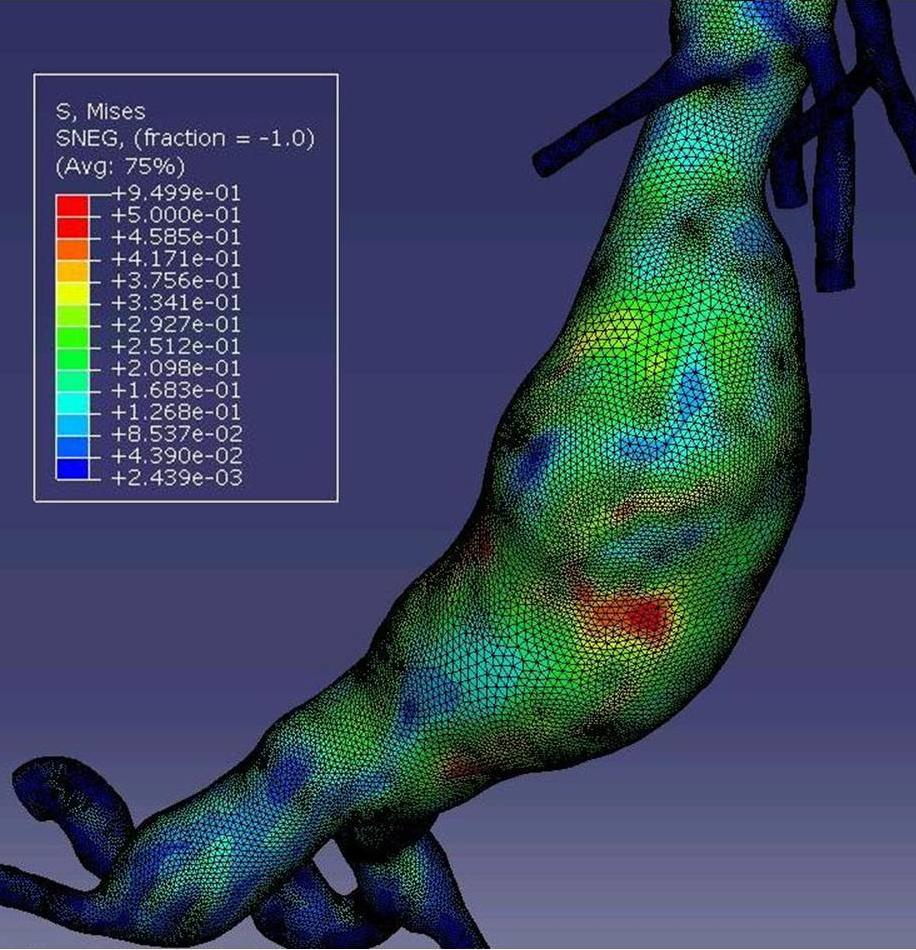
\includegraphics[width=0.382\textwidth]{pictures/aneurysma}
  \end{center}
%\caption{A gull}
\end{wrapfigure}
Um Lösungen zu Differentialgleichungen zu finden, Trajektorien und zeitabhängige Graphen zu plotten, sind wir auf die Hilfe von leistungsstarken Computern und Software angewiesen.

Es gibt zahlreiche numerische Verfahren zur Bestimmung von Ableitungen, Integralen, Summen etc. Wir wollen uns im Folgenden einen Auszug aus der Vielfalt der Verfahren anschauen und kurz auf deren Genauigkeit abschätzen.

\subsection{Numerische Standardverfahren}

Wir betrachten eine Differentialgleichung der Form
$$y'=f(t,y)$$
mit Startwert $y_0=y(t_0)$ und wenden darauf die folgenden Verfahren an, um $y(t)$ über einem Zeitintervall $t_0<t<T$ numerisch abzuschätzen.

Wir beginnen mit einer simplen Methode, dem Euler-Verfahren, um die grundsätzliche Idee eines Näherungsverfahren zu erfassen und besprechen dann eine weit verbreitete Methode, das Runge-Kutta-Verfahren.

\subsubsection{Das Euler-Verfahren}

Klar ist, dass ein Computer nicht jeden Punkt einer Kurve berechnen kann, weil es ja unendlich viele davon gibt. Also beschränkt sich ein Näherungsverfahren immer auf eine diskrete Teilmenge. Euler's Methode beschreibt eine sehr einfache Annäherung an die Lösung einer Differentialgleichung für eine endliche Anzahl von Punkten. Die Teilschritte sind

\begin{enumerate}
\item Teile das betrachtete Intervall in $N$ gleich grosse Abschnitte und setze für $n=0,1,2,\dots,N-1$
$$t_n=t_0+nh,$$
wobei $h=\frac{T-t_0}{N}$ die Schrittweite ist.
\item Ausgehend vom Punkt $(t_0|y_0)$ auf der Kurve approximiert man $y_n=y(t_n)$. Eine Näherung für $y_1$ bestimmen wir via der Tangente durch $(t_0|y_0)$ bis $t_1$. Also
$$y_1\approx y_0+hf(t_0,y_0)$$
mit
$$y'=f(t_0,y_0)\approx\frac{y_1-y_0}{h}=\frac{y_1-y_0}{t_1-t_0}.$$
\item Bestimme so $y_2\approx y_1+f(t_1,y_1)$ und weiter $y_3,\dots,y_n$.
\end{enumerate}

Allgemein beschrieben hat man das rekursive Schema
$$y_{n+1}=y_n+hf(t_n,y_n)$$
mit
$$t_{n+1}=t_n+h$$
für $0\leq n\leq N-1$.

\begin{figure}
\begin{center}
\scalebox{1.3}{
\begin{tikzpicture}[line cap=round,line join=round,>=triangle 45,x=0.82cm,y=0.82cm]
\draw[->,color=black] (-0.88,0) -- (7.62,0);
\foreach \x in {,1,2,3,4,5,6,7}
\draw[shift={(\x,0)},color=black] (0pt,-2pt);
\draw[color=black] (7.34,0.08) node [anchor=south west] {$t$};
\draw[->,color=black] (0,-1.2) -- (0,4.44);
\foreach \y in {-1,1,2,3,4}
%\draw[shift={(0,\y)},color=black] (2pt,0pt) -- (-2pt,0pt);
\draw[color=black] (0.1,4.04) node [anchor=west] {$y$};
\clip(-0.88,-1.2) rectangle (7.62,4.44);
\draw plot[raw gnuplot, id=func0] function{set samples 100; set xrange [0:2]; plot 1};
\draw plot[raw gnuplot, id=func1] function{set samples 100; set xrange [2:4]; plot 0.2*x+0.6};
\draw plot[raw gnuplot, id=func2] function{set samples 100; set xrange [4:6]; plot 0.4*x-0.2};
\draw plot[raw gnuplot, id=func3] function{set samples 100; set xrange [6:7]; plot 0.6*x-1.4};
\draw plot[raw gnuplot, id=func4] function{set samples 100; set xrange [0:7]; plot 0.05*x**2+1};
\draw (3.36,2.82) node[anchor=north west] {Lösung};
\draw (5.62,2.1) node[anchor=north west] {Euler};
\draw (-0.8,1.38) node[anchor=north west] {$y_0$};
\draw (0.06,0) node[anchor=north west] {$t_0$};
\draw (2.06,0) node[anchor=north west] {$t_1$};
\draw (4.06,0) node[anchor=north west] {$t_2$};
\draw (6.06,0) node[anchor=north west] {$t_3$};
\end{tikzpicture}
}
\end{center}
\caption{Das Euler-Verfahren}
\end{figure}

\begin{bsp}
Wir bestimmen mit dem Euler-Verfahren mit Schrittweite $h=0.1$ eine Näherung für $y(0.2)$ der Gleichung
$$\frac{\mathrm{d}y}{dt}=y^2+t$$
mit Startwert $y(0)=1$.

Hier ist $f(t,y)=y^2+t$. Für $n=0$ ist
$$y_1=y(0.1)=y_0+hf(t_0,y_0)=1.1.$$
Mit $n=1$ erhalten wir
$$y_2=y(0.2)=y_1+hf(t_1,y_1)=1.231.$$
\end{bsp}

Vergleichen wir die Taylor-Entwicklung von
$$y_{n+1}=y_n+h\frac{\mathrm{d}y_n}{dt}+\frac{h^2}{2!}\frac{d^2y_n}{dt^2}+\dots$$
mit der Euler-Methode, so sehen wir, dass letztere aus den ersten zwei Summanden besteht. Man sagt: Das Euler-Verfahren ist eine first-order Approximation. Nun versuchen wir aufgrund dieser Beobachtung den Fehler abzuschätzen und möglicherweise durch Anpassung der Schrittweite den Fehler zu kontrollieren.

Euler liefert den Näherungswert
$$y_{n+1}=y_n+hf(t_n,y_n)$$
und Taylor den wahren Wert
$$y(t_{n+1})=y(t_n)+hf(t_n,y(t_n))+\frac{h^2}{2}f'(\zeta,y(\zeta_n))$$
wobei $\zeta_n$ zwischen $t_n$ und $t_{n+1}$ liegt. Subtrahieren wir Euler von Taylor erhalten wir den Fehlerterm
$$
E_{n+1}=y(t_n)-y_n+
h(f(t_n,y(t_n))-f(t_n,y_n))+\frac{h^2}{2}f'(\zeta_n,y(\zeta_n)).
$$
Man kann zeigen, dass dieser Fehlerterm durch
$$E_{n+1}\leq \frac{Dh}{2L}(\mathrm{e}^{T-t_0}-1)$$
nach oben beschränkt ist, wobei $L$ eine obere Schranke für $f$ und $D$ eine obere Schranke für $f'$ über dem Intervall $[t_0,T]$ ist und $f$ gutmütig sowie $T=t_0+(N-1)h$.

Wegen $\lim_{h\to0}E_{n+1}=0$ liegt die Vermutung nahe, dass die Genauigkeit mit kleiner werdenden Schrittweite zunimmt.

\subsubsection{Das Runge-Kutta-Verfahren}

One-step Algorithmen, die durchschnittliche Steigungen einer Funktion $f(t,y)$ in zwei oder mehreren Punkten über einem Intervall $[t_{n-1},t_n]$ verwenden um $y_n$ zu berechnen, heissen Runge-Kutta Methoden.

Eine weit verbreitete Methode ist das Runge-Kutta-Verfahren vierter Ordnung (RK4). Es verwendet gewichtete durchschnittliche Steigungen um die Mittel- und Endpunkte von Teilintervallen. algorithmisch formuliert
$$y_{n+1}=y_n+\frac{h}{6}(k_1+2k_2+2k_3+k_4)$$
mit
\begin{align*}
k_1 &= f(t_n,y_n)\\
k_2 &= f(t_n+\frac{h}{2},y_n+\frac{h}{2}k_1)\\
k_3 &= f(t_n+\frac{h}{2},y_n+\frac{h}{2}k_2)\\
k_4 &= f(t_n+h,y_n+hk_3)
\end{align*}

\clearpage

\section{Ein Raketenmodell}
\begin{figure}
  \begin{center}
    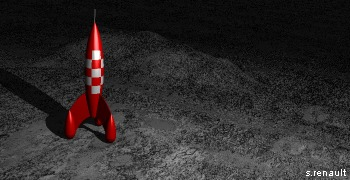
\includegraphics[width=0.618\textwidth]{pictures/raketetim}
  \end{center}
%\caption{A gull}
\end{figure}

\subsection{Das Pfupfmodell}

Wir betrachten das klassische \enquote{Pfupfmodel} einer Rakete der Masse $m$ mit Geschwindigkeit $v$ und verwenden den Impulserhaltungssatz. Wir notieren also jeweils den Impuls $p$ vor und nach dem Stoss und vergleichen.

\begin{figure}[h!]
  \begin{center}
    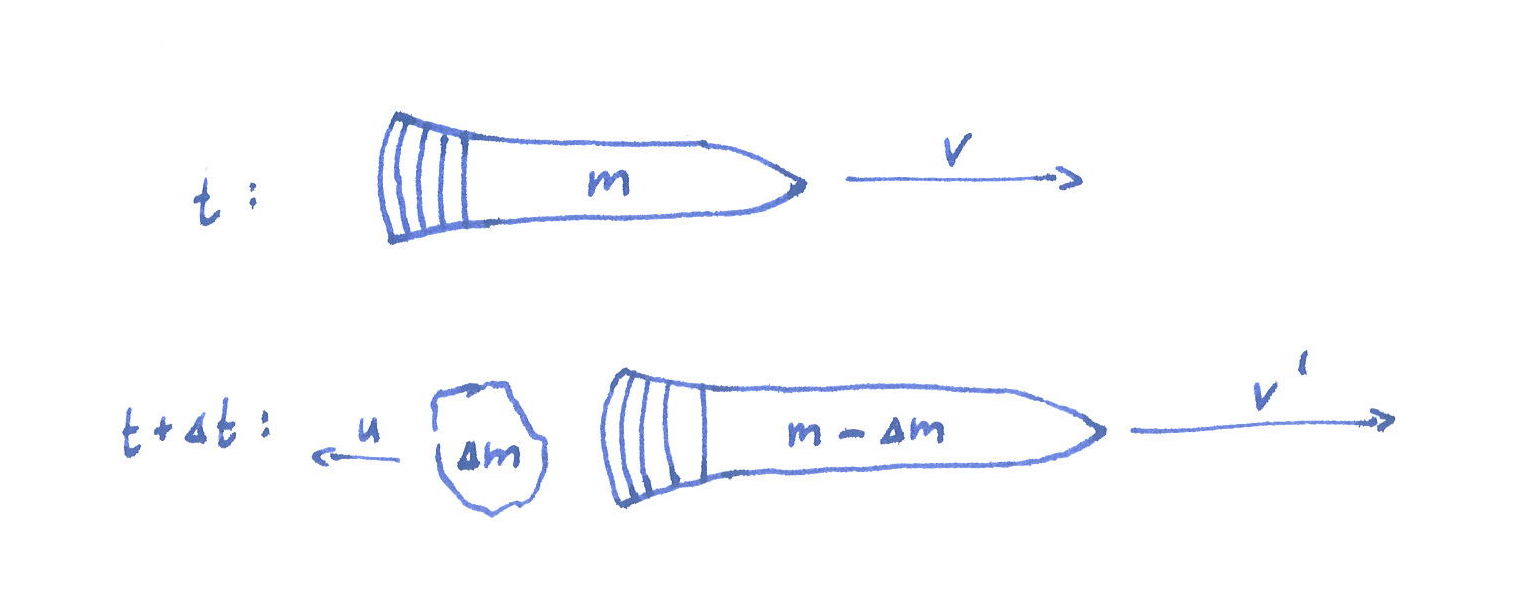
\includegraphics[width=0.618\textwidth]{pictures/raketeimpuls}
  \end{center}
\caption{Pfupf-Modell einer Rakete}
\end{figure}

Mit obiger Notation gilt nach dem Pfupf:
$$p=(m-\Delta m)\cdot v'+\Delta m\cdot(v'-v_g)$$
und unmittelbar folgt mit $p=mv$ vor dem Pfupf
$$mv=mv'-\Delta mu,$$
wobei $v'$ die Geschwindigkeit der Rakete nach dem Stoss und $v_g$ die Ausströmgeschwindigkeit des Gases bezeichnet.

Berechnen wir damit den Geschwindigkeitsverlauf der Rakete. Wir lösen
$$mv=mv'-\Delta mv_g$$
nach $v'-v$ und bezeichnen diese Geschwindigkeitszunahme mit $\Delta v$:
$$\Delta v=\frac{\Delta mv_g}{m}.$$
Mit Division und für $\Delta t\to0$ erhalten wir die Differentialgleichung
$$\mathrm{d}v=-\frac{\mathrm{d}m}{m}\cdot v_g.$$
Das Vorzeichen erklärt sich dadurch, dass die Geschwindigkeit zunimmt, wenn Masse abnimmt. Wir integrieren, um die Geschwindigkeit zu erhalten:
$$\int_{v_0}^v\,\mathrm{d}v=\int_{m_0}^m-\frac{v_g}{m}\,\mathrm{d}m.$$
Also gilt für die Geschwindigkeit der Rakete mit Anfangsmasse $m_0$ und Anfangsgeschwindigkeit $v_0$
$$v(t)=v_0+v_g\cdot\ln\left(\frac{m_0}{m}\right).$$
Dieser Ausdruck wird auch \definition{1. Raketengleichung} genannt. Sie gibt die Geschwindigkeit einer Rakete im Vakuum ohne Gravitationseinfluss an.

\subsection{Geschwindigkeitsverlauf}

Wir wollen das $v$-$t$-Diagramm zeichnen. Dazu müssen wir beachten, dass $m$ auch von der Zeit abhängt, $m=m(t)$.
$$v(t)=v_0+v_g\cdot\ln\left(\frac{m_0}{m(t)}\right).$$
Nehmen wir einen zeitlich konstanten Gasausstoss $\mu$ an, so gilt für die Masse der Rakete zur Zeit $t$
$$m(t)=m_0-\mu t$$
und damit für die Geschwindigkeit
$$v(t)=v_0+v_g\cdot\ln\left(\frac{m_0}{m_0-\mu t}\right).$$

So, setzen wir $v_0=0$, $u=2500$, $m_0=2200$ und $\mu=2.5$ und schauen uns Abbildung \ref{geschwindigkeitrakete} an.

\begin{figure}
\definecolor{cqcqcq}{rgb}{0.7529,0.7529,0.7529}
\begin{center}
\begin{tikzpicture}[line cap=round,line join=round,>=triangle 45,x=0.01cm,y=0.00065cm]
\draw [color=cqcqcq,dash pattern=on 3pt off 3pt, xstep=1.0cm,ystep=1.31cm] (0,0) grid (900.,9900);
\draw[->,color=black] (-100.,0.) -- (900.,0.);
\foreach \x in {100,200,300,400,500,600,700,800}
\draw[shift={(\x,0)},color=black] (0pt,2pt) -- (0pt,-2pt) node[below] {\footnotesize $\x$};
\draw[color=black] (872.413793103,89.172) node [anchor=south west] { t};
\draw[->,color=black] (0.,-100.) -- (0.,10000.0028571);
\foreach \y in {2000,4000,6000,8000}
\draw[shift={(0,\y)},color=black] (2pt,0pt) -- (-2pt,0pt) node[left] {\footnotesize $\y$};
\draw[color=black] (8.62068965517,9509.55685714) node [anchor=west] { v(t)};
\clip(-100.,-500.000142857) rectangle (900.,10000.0028571);
\draw[line width=1.2pt,smooth,samples=100,domain=0:865.0000000000001] plot(\x,{2500.0*ln(2200.0/(2200.0-2.5*(\x)))});
\begin{scriptsize}
\end{scriptsize}
\end{tikzpicture}
\end{center}
\caption{Geschwindigkeitsverlauf der Rakete}\label{geschwindigkeitrakete}
\end{figure}


Man sieht, dass die Rakete immer stärker beschleunigt. So lange, bis der Brennstoff aufgebraucht ist. Wie lange dauert das? Um diese Frage zu beantworten, nehmen wir uns $m_0$ vor und schreiben
$$m_0=m_{leer}+m_{brenn}.$$
Dabei ist natürlich zu beachten, dass $m_{leer}$ inklusive Nutzlast aufzufassen ist. Ist zum Beispiel $m_{leer}=200$, so erhält man für $m_{brenn}=\mu\cdot t_{brenn}$ die Brenndauer
$$t_{brenn}=\frac{m_{brenn}}{\mu}.$$
Für obige Werte hat man $t_{brenn}=\unit[800]{Sekunden}$.

\subsection{Brennschlussgeschwindigkeit}

Von Interesse ist auch, welche Endgeschwindigkeit die Rakete erreicht. Wir setzen also im Geschwindigkeitsverlauf $m_0=m_{leer}$, da ja kein Brennstoff mehr vorhanden ist. Numerisch ergibt sich
$$v_e=v_0+v_g\cdot\ln\left(\frac{m_0}{m_{leer}}\right)\approx\unitfrac[6000]{m}{s}$$

Man will die Endgeschwindigkeit optimieren. Sie ist proportional zur Ausströmgeschwindigkeit und hängt logarithmisch vom Verhältnis Masse beim Start zu Masse nach Brennschluss ab. Mehr Erkenntnis gibt unser Model nicht her.

\subsection{Nutzlasten}

Will man Material in eine Umlaufbahn bringen, so muss man grosse Endgeschwindigkeiten erreichen können. Wir betrachten, wiederum für $v_0=0$, das Verhältnis von Endgeschwindigkeit zu Gasgeschwindigkeit:
$$\frac{v_e}{v_g}=\ln\left(\frac{m_0}{m_{leer}}\right)=\ln\left(1+\frac{m_{brenn}}{m_{leer}}\right).$$
Also ist der Zusammenhang vom Typ
$$v_v=\ln(1+m_v)$$
mit $v_v=\frac{v_e}{v_g}$ und $m_v=\frac{m_{brenn}}{m_{leer}}$ oder in der Anschauung in Abbildung \ref{raketeverhaeltnis}.

\begin{figure}
\definecolor{cqcqcq}{rgb}{0.752941176471,0.752941176471,0.752941176471}
\begin{center}
\begin{tikzpicture}[line cap=round,line join=round,>=triangle 45,x=0.15cm,y=1.2cm]
\draw [color=cqcqcq,dash pattern=on 2pt off 2pt, xstep=1.5cm,ystep=1.2cm] (0,0) grid (65.7327586207,4.8);
\draw[->,color=black] (-5.,0.) -- (65.7327586207,0.);
\foreach \x in {10,20,30,40,50,60}
\draw[shift={(\x,0)},color=black] (0pt,2pt) -- (0pt,-2pt) node[below] {\footnotesize $\x$};
\draw[color=black] (63.0172413793,0.0509554140127) node [anchor=south west] { $m_v$};
\draw[->,color=black] (0.,-0.5) -- (0.,5.);
\foreach \y in {1,2,3,4}
\draw[shift={(0,\y)},color=black] (2pt,0pt) -- (-2pt,0pt) node[left] {\footnotesize $\y$};
\draw[color=black] (0.646551724138,4.65605095541) node [anchor=west] { $v_v$};
\draw[color=black] (0pt,-10pt) node[right] {\footnotesize $0$};
\clip(-5.,-0.859872611465) rectangle (65.7327586207,5.);
\draw[smooth,samples=100,domain=0.00001:65.73275862068971] plot(\x,{ln(1.0+(\x))});
\begin{scriptsize}
\end{scriptsize}
\end{tikzpicture}
\end{center}
\caption{Verhältnisgleichung für Nutzlasten}\label{raketeverhaeltnis}
\end{figure}

Selbst bei einem Verhältnis von $50$ von Brennstoff zu Leermasse erhält man nur eine $4$mal so grosse Endgeschwindigkeit wie die Ausströmgeschwindigkeit.

\begin{bem}
Es ist ressourcenverschlingend, grosse Nutzlasten auf hohe Endgeschwindigkeiten zu bringen.
\end{bem}

Folgend einige Werte von Ausströmgeschwindigkeiten, die heute erreicht werden können:
\begin{description}
\item Feststoffrakete  $\unitfrac[2000]{m}{s}$
\item Flüssigbrennstoffrakete  $\unitfrac[3200]{m}{s}$
\item Hybride  $\unitfrac[4000]{m}{s}$
\end{description}

Welche Geschwindigkeit muss eine Rakete erreichen, um das Gravitationsfeld der Erde zu verlassen (Fluchtgeschwindigkeit). Mit Energieerhaltung
$$G\cdot\frac{Mm}{r}=\frac{1}{2}mv_2^2$$
erhält man
$$v_2=\sqrt{\frac{2GM}{r}}.$$
Um den Einflussbereich der Erde zu verlassen, muss eine Rakete eine Geschwindigkeit von $\unitfrac[11.2]{km}{s}$ haben.

\begin{bem}
Die konstruktive Obergrenze für eine einstufige Rakete liegt bei $15\div1$, womit klar ist, dass man mit einer einstufigen Rakete die Fluchtgeschwindigkeit (auch 2. kosmische Geschwindigkeit) nicht erreichen kann.
\end{bem}

\subsection{Rakete unter konstantem Schwerkrafteinfluss}

Für einen senkrechten Wurf nach oben gilt
$$v(t)=v_0-gt$$
und somit für die Rakete
$$v(t)=v_g\cdot\ln\left(\frac{m_0}{m_0-\mu t}\right)-gt.$$
Mit den Werten $v_g=1000$, $m_0=1100$, $\mu=10$, $g=9.81$ berechnen wir noch die Brenndauer $t'$ via
$$m_{brenn}=\mu t'$$
und finden $t'=100$.
Nach Brennschluss haben wir
$$v(t)=v_{brenn}-gt$$
wobei $v_{brenn}$ die Brennschlussgeschwindigkeit bezeichnet. Da dieser Geschwindigkeitsverlauf erst nach Brennschluss stattfindet, verschieben wir die Funktion um die Zeit $t'$
$$v_{nach}(t)=v(t')-g(t-t')$$
Insgesamt haben wir
$$\tilde{v}(t)=
\begin{cases}
v(t)& t<t'\\
v_{nach}(t)& t\geq t'
\end{cases}
$$
Der Graph sieht folgendermassen aus:

\begin{figure}[h!]
\definecolor{cqcqcq}{rgb}{0.7529,0.7529,0.7529}
\begin{center}
\begin{tikzpicture}[line cap=round,line join=round,>=triangle 45,x=0.03cm,y=0.003cm]
\draw [color=cqcqcq,dash pattern=on 2pt off 2pt, xstep=1.5cm,ystep=0.6cm] (0,0) grid (300,1900);
\draw[->,color=black] (-30.,0.) -- (300.,0.);
\foreach \x in {50,100,150,200,250}
\draw[shift={(\x,0)},color=black] (0pt,2pt) -- (0pt,-2pt) node[below] {\footnotesize $\x$};
\draw[color=black] (290.896551724,18.6836668966) node [anchor=south west] { t};
\draw[->,color=black] (0.,-30.) -- (0.,2000.00148915);
\foreach \y in {200,400,600,800,1000,1200,1400,1600,1800}
\draw[shift={(0,\y)},color=black] (2pt,0pt) -- (-2pt,0pt) node[left] {\footnotesize $\y$};
\draw[color=black] (2.84482758621,1897.24132122) node [anchor=west] { v(t)};
\draw[color=black] (0pt,-10pt) node[right] {\footnotesize $0$};
\clip(-30.,-200.000287915) rectangle (300.,2000.00148915);
\draw[line width=1.2pt,smooth,samples=100,domain=0:100] plot(\x,{1000.0*ln(1100.0/(1100.0-10.0*(\x)))-9.81*(\x)});
\draw[line width=1.0pt,smooth,samples=100,domain=100:244.444] plot(\x,{2398.0-9.81*(\x)});
\begin{scriptsize}
\end{scriptsize}
\end{tikzpicture}
\end{center}
\end{figure}

Wie hoch steigt bei diesem Geschwindigkeitsverlauf die Rakete? Wir bestimmen den Steigungsverlauf als Integral über den Geschwindigkeitsverlauf:
$$s(t)=\int_0^t\tilde{v}(\tau)\,\mathrm{d}\tau.$$
Vor Brennschluss haben wir
$$s(t)=\int \left[v_g\cdot\ln\left(\frac{m_0}{m_0-\mu t}\right)-gt\right]\,\mathrm{d}t$$
und danach
$$s(t)=\int \left[v(t')-g(t-t')\right]\,\mathrm{d}t.$$
Kompakt formuliert

$$\tilde{s}(t)=
\begin{cases}
-\frac{g}{2}t^2+v_gt+v_g(t-\frac{m_0}{\mu})\cdot\ln\left(\frac{m_0}{m_0-\mu t}\right)& t<t'\\
-\frac{g}{2}t^2+(gt'+v(t'))t& t\geq t'
\end{cases}
$$

\clearpage

\section{Spezielle Potenzreihen}

\subsection{Die Hermite'sche Differentialgleichung}

Betrachte
\begin{equation}\label{eq:hermit}
y''-2xy'+\lambda y=0
\end{equation}
mit $\lambda\in\mathbb{R}$. Mit dem Potenzreihenansatz
$$y(x)=\sum_{k=0}^\infty c_k\cdot x^k$$
erhalten wir die Bedingung
$$
(2c_2+\lambda c_0)
+\sum_{k=1}^\infty[(k+1)(k+2)c_{k+2}-2kc_k+\lambda c_k]\cdot x^k=0,
$$
die wir wie folgt erfüllen können. $c_0$ und $c_1$ können frei gewählt werden, und für $k\geq0$ muss
$$c_{k+2}=\frac{2k-\lambda}{(k+1)(k+2)}\cdot c_k$$
gelten. So erhalten wir
$$y(x)=c_0g(x)+c_1h(x)$$
mit
$$
g(x)=1-\frac{\lambda}{2!}x^2
-\sum_{k=2}^\infty\frac{[4(k-1)-\lambda][4(k-2)-\lambda]\dotsm[4-\lambda]\lambda}{(2k)!}\cdot x^{2k}
$$
und
$$
h(x)=x
+\sum_{k=1}^\infty\frac{[4k-2-\lambda][4(k-1)-2-\lambda]\dotsm[2-\lambda]}{(2k+1)!}\cdot x^{2k+1}.
$$
Besonders interessant ist der Fall $\lambda=2n$ für $n\in\mathbb{N}_0$. Wenn $n$ gerade ist, ist in diesem Fall $g=g_n$ ein gerades Polynom vom Grad $n$; wenn $n$ ungerade ist, ist $h=h_n$ ein ungerades Polynom vom Grad $n$. Man definiert die \definition{Hermite'schen Polynome} $H_n$ durch
$$H_n=(-1)^{n/2}\cdot2^{n/2}\cdot3\cdot5\dotsm(n-1)\cdot g_n,$$
für gerade $n$ und
$$H_n=(-1)^{(n-1)/2}\cdot2^{(n+1)/2}\cdot3\cdot5\dotsm n\cdot h_n,$$
falls $n$ ungerade ist.

\begin{uebenv}{hermitepoly}
Kannst du die ersten paar Hermite'schen Polynome, vielleicht $H_0$ bis $H_3$, bestimmen?
\end{uebenv}

\begin{bem}
Es wird gesagt, die Differentialgleichung \eqref{eq:hermit} trete in der Quantentheorie beim Studium der Schwingungen von Molekülen auf.
\end{bem}


\subsection{Die Legendre'sche Differentialgleichung}

Sie hat ihren Ursprung in der Astronomie und lautet
\begin{equation}\label{eq:legendre}
(1-x^2)y''-2xy'+\lambda(\lambda+1)y=0.
\end{equation}
Wir suchen eine Potenzreihenentwicklung $y(x)$ um $x_0=0$. Weil sich die Funktionen
$$x\mapsto\frac{-2x}{1-x^2}\quad\text{und}\quad x\mapsto\frac{\lambda(\lambda+1)}{1-x^2}$$
über dem Intervall $(-1,1)$ in Potenzreihen entwickeln lassen, lässt sich über diesem Intervall die Differentialgleichung durch eine Potenzreihe auflösen.
Wir beginnen mit
$$y(x)=\sum_{k=0}^\infty c_k\cdot x^k$$
und der Abkürzung $\lambda(\lambda+1)=\alpha$. Eine kleine Rechnung führt zur Rekursionsformel
$$c_{k+2}=\frac{k(k+1)-\alpha}{(k+1)(k+2)}\cdot c_k$$
mit $k\in\mathbb{N}_0$. Wir können $c_0$ und $c_1$ frei wählen und erhalten die Werte für $c_k, k\geq2$ mit obiger Formel. Dies führt zu
$$y(x)=c_0g(x)+c_1h(x)$$
mit
$$
g(x)=1-\frac{\lambda(\lambda+1)}{2}x^2
-\sum_{k=2}^\infty\frac{\lambda(\lambda+1)}{2k}\left(1-\frac{\lambda(\lambda+1)}{2\cdot3}\right)
\dots \cdot \left(1-\frac{\lambda(\lambda+1)}{(2k-2)(2k-1)}\right) x^{2k}
$$
und
$$
h(x)=x
+\sum_{k=1}^\infty\frac{1}{2k+1}\left(1-\frac{\lambda(\lambda+1)}{1\cdot2}\right)
\dots\cdot \left(1-\frac{\lambda(\lambda+1)}{(2k-1)(2k)}\right) x^{2k+1}.
$$
Wieder interessiert der Fall $\lambda=n\in\mathbb{N}$ besonders. Wenn $n$ gerade ist, setzen wir $p_n=g_n$; wenn $n$ ungerade ist, setzen wir $p_n=h_n$. Das \definition{Legendre-Polynom} ist gegeben durch $P_n=\alpha_np_n$, wobei $\alpha$ so bestimmt werden soll, dass der Koeffizient des Monoms $x^n$ in $P_n$ den Wert $\frac{(2n)!}{2^n(n!)^2}$ annimmt. $P_n$ ist dann eine Lösung der Legendre'schen Differentialgleichung.

\subsection{Die Tschebyscheff'sche Differentialgleichung}

Sie ging aus dem Studium der Kolbenbewegung in Dampfmaschinen hervor und lautet
$$(1-x^2)y''-xy'+\lambda^2y=0.$$
Sie kann ähnlich wie die Legendre-Gleichung durch einen Potenzreihenansatz über dem Intervall $(-1,1)$ gelöst werden und führt zu den \emph{Tschebyscheff-Polynomen}.

\begin{lsg}{hermitepoly}
    $H_0=g_0=1$, $H_1=h_1=2x$, $H_2=(-1)\cdot2(1-\frac{4}{2!}x^2=-2+4x^2$, $H_3=(-1)\cdot 2^2\cdot3(x+\frac{-24}{3!}x^3=-12x+8x^3$
\end{lsg}

\cleardoublepage
\listoffigures
%\listoftables
%\newpage
%\nocite{*}
%\bibliographystyle{plain}
%\bibliography{preamble/literaturgoogle}
\end{document}